\documentclass[10pt]{beamer}

\usetheme[progressstyle=movingCircCnt]{Feather}

\usepackage[utf8]{inputenc}
\usepackage[T1]{fontenc}
\usepackage{helvet}
\usepackage{booktabs}
\usepackage{array}
\usepackage{ragged2e}
\usepackage{tikz}
\usetikzlibrary{arrows.meta,positioning,calc}

\graphicspath{{assets/}}

\definecolor{UnBBlue}{RGB}{0,51,102}
\definecolor{UnBGreen}{RGB}{33,140,33}
\definecolor{SoftBlue}{RGB}{230,239,247}
\definecolor{SoftGreen}{RGB}{231,244,231}
\definecolor{SoftRed}{RGB}{250,232,232}
\definecolor{TextGray}{RGB}{84,97,110}

\setbeamercolor{Feather}{fg=UnBGreen,bg=UnBBlue}
\setbeamercolor{structure}{fg=UnBBlue}
\setbeamercolor{frametitle}{fg=white,bg=UnBBlue}
\setbeamercolor{normal text}{fg=TextGray,bg=white}
\setbeamercolor{alerted text}{fg=UnBGreen}
\setbeamercolor{block title}{fg=white,bg=UnBBlue}
\setbeamercolor{block body}{fg=TextGray,bg=SoftBlue}
\setbeamertemplate{caption}{\raggedright\insertcaption\par}
\setbeamertemplate{navigation symbols}{}

\newcommand{\source}[1]{%
  \par\vfill{\raggedleft\tiny\color{gray}Fonte: #1\par}%
}

\newcommand{\keynumber}[2]{%
  {\color{UnBBlue}\bfseries\LARGE #1}\par
  {\small #2}%
}

\newcommand{\modelwinner}[3]{%
  \textbf{#1}\hfill{\color{UnBGreen}\textbf{#2}}\par
  {\scriptsize #3}\par\vspace{0.35em}%
}

\title[Predição de interrupções na rede elétrica do DF]
{\textbf{Predição de Interrupções no Fornecimento de Energia Elétrica no Distrito Federal:}}

\subtitle[]
{\textbf{Um estudo comparativo entre XGBoost e redes neurais recorrentes bidirecionais}}

\author[Giovanni Zanetti e Mateus Araújo]
{Giovanni Minari Zanetti \and Mateus Gomes de Araújo}

\institute[]
{Instituto de Ciências Exatas -- Departamento de Ciência da Computação\\
Curso de Engenharia de Computação\\[2mm]
Orientador: Prof. Jan Mendonça Corrêa}

\date{Brasília, 2026}

\begin{document}

% ------------------------------------------------------------------
% ABERTURA — Giovanni
% ------------------------------------------------------------------

{\1
\begin{frame}[plain,noframenumbering]
  \titlepage
  \note{%
    Apresentador: Giovanni. Tempo-alvo: 30 segundos.
    Cumprimentar a banca, apresentar os autores e enunciar o tema.
    [Sources] Monografia, elementos pré-textuais.
  }
\end{frame}}

\section{Problema e objetivo}

\begin{frame}{Podemos antecipar as interrupções?}{Pergunta de pesquisa}
  \vspace{0.5em}
  \begin{block}{}
    \centering
    \Large
    Dados públicos de clima e operação conseguem prever quantas interrupções ocorrerão nos próximos dias?
  \end{block}

  \vspace{0.7em}
  \begin{itemize}
    \item \textbf{Alvo:} número diário de interrupções no Distrito Federal.
    \item \textbf{Comparação:} XGBoost, Bi-LSTM e Bi-GRU.
    \item \textbf{Horizontes:} 1, 3, 7 e 14 dias à frente.
  \end{itemize}

  \source{Monografia, Capítulo 1.}
  \note{%
    Apresentador: Giovanni. Tempo-alvo: 1 minuto.
    Abrir com a pergunta central e explicar que o trabalho combina previsão diária e análise multi-horizonte.
    [Sources] Monografia, Seções 1.1 e 1.2.
  }
\end{frame}

\begin{frame}{Interrupções cresceram 65,3\% desde 2017}{Contexto operacional}
  \begin{columns}[T,onlytextwidth]
    \begin{column}{0.72\textwidth}
      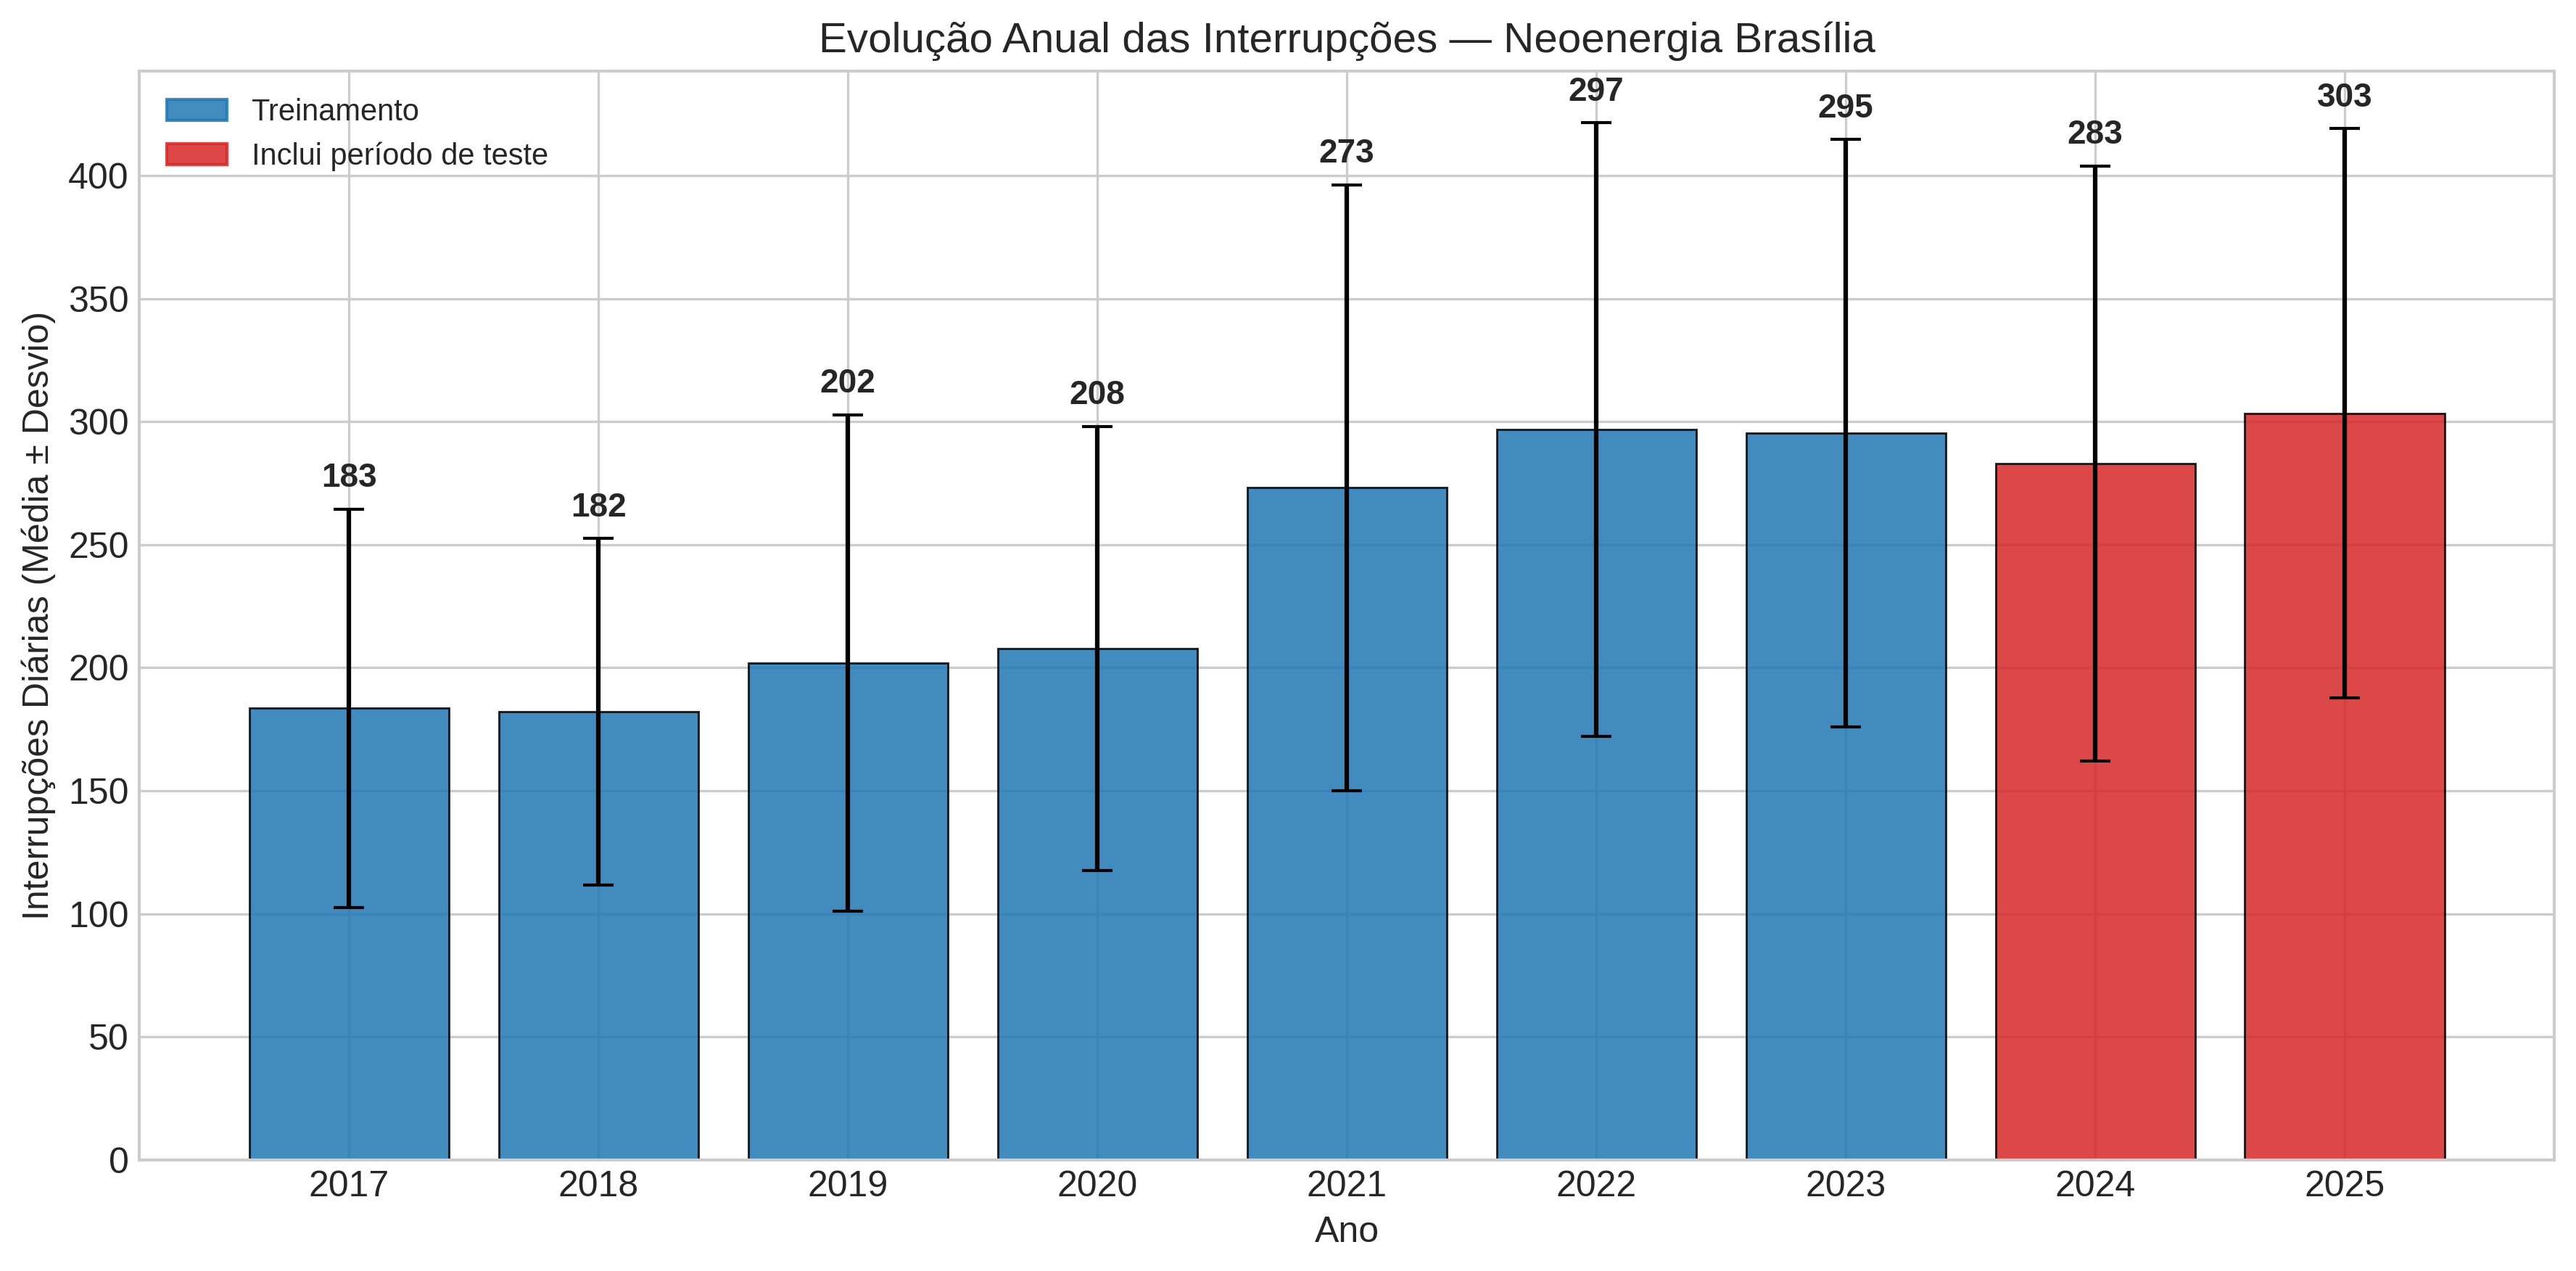
\includegraphics[width=\textwidth]{evolucao_anual_interrupcoes.png}
    \end{column}
    \begin{column}{0.25\textwidth}
      \vspace{1.0em}
      \keynumber{183,5}{interrupções/dia em 2017}
      \vspace{1.0em}
      \keynumber{303,4}{interrupções/dia em 2025}
      \vspace{1.0em}
      \keynumber{1.424}{pior dia observado}
      \vspace{0.6em}
      {\scriptsize 2025 contém dados de janeiro a maio.}
    \end{column}
  \end{columns}

  \source{ANEEL; elaboração dos autores, 2017--2025.}
  \note{%
    Apresentador: Giovanni. Tempo-alvo: 1 minuto e 20 segundos.
    Ressaltar que 2025 contém janeiro a maio e que o crescimento é descritivo, não causal.
    [Sources] Monografia, Seções 1 e 3.7; Figura 4.2.
  }
\end{frame}

\begin{frame}{Prever picos permite agir antes da falha}{Motivação}
  \vspace{0.4em}
  \begin{columns}[T,onlytextwidth]
    \begin{column}{0.47\textwidth}
      \textbf{\large Cenário atual}
      \begin{itemize}
        \item Redes aéreas de 13,8 kV expostas ao clima do Cerrado.
        \item Chuvas intensas, rajadas e calor pressionam a infraestrutura.
        \item Resposta predominantemente reativa após a interrupção.
      \end{itemize}
    \end{column}
    \begin{column}{0.47\textwidth}
      \textbf{\large Oportunidade}
      \begin{itemize}
        \item Pré-posicionar equipes e materiais.
        \item Planejar comunicação e contingência.
        \item Apoiar uma manutenção orientada por risco.
      \end{itemize}
    \end{column}
  \end{columns}

  \vspace{0.8em}
  \begin{block}{}
    \centering
    A previsão não elimina a incerteza, mas transforma histórico e clima em antecedência operacional.
  \end{block}

  \source{Monografia, Seções 1.1 e 5.6.}
  \note{%
    Apresentador: Giovanni. Tempo-alvo: 1 minuto.
    Conectar o problema técnico à decisão operacional.
    [Sources] Monografia, Justificativa e Implicações Práticas.
  }
\end{frame}

\begin{frame}{O trabalho entrega quatro contribuições}{Contribuições}
  \begin{enumerate}
    \item \textbf{Base diária integrada}\\
      3.073 dias de clima e interrupções; consumo mensal do SAMP usado apenas na análise exploratória.
    \item \textbf{Memória temporal explícita}\\
      40 atributos derivados com defasagens, médias móveis, variabilidade e sazonalidade.
    \item \textbf{Comparação equânime}\\
      365 dias em $h=1$ e 352 datas causais comuns na análise multi-horizonte.
    \item \textbf{Escolha por horizonte}\\
      Desempenho comparado em previsões diretas de 1, 3, 7 e 14 dias.
  \end{enumerate}

  \source{Monografia, Seção 1.4.}
  \note{%
    Apresentador: Giovanni. Tempo-alvo: 1 minuto e 10 segundos.
    Apresentar as contribuições como respostas concretas à pergunta de pesquisa.
    [Sources] Monografia, Seção 1.4.
  }
\end{frame}

\section{Dados e metodologia}

\begin{frame}{Duas bases preditivas e uma exploratória}{Dados e escopo}
  \begin{columns}[T,onlytextwidth]
    \begin{column}{0.61\textwidth}
      \begin{description}
        \item[INMET] temperatura, precipitação, velocidade, rajada e direção do vento.
        \item[ANEEL] registros de interrupções e fatores geradores.
        \item[SAMP] consumo mensal de energia, usado somente na análise exploratória.
      \end{description}
    \end{column}
    \begin{column}{0.34\textwidth}
      \keynumber{2017--2025}{período analisado}
      \vspace{0.8em}
      \keynumber{3.073}{dias brutos}
      \vspace{0.8em}
      \keynumber{3.066}{observações finais}
    \end{column}
  \end{columns}

  \vspace{0.5em}
  \begin{block}{Delimitação}
    Distribuição de energia no DF, resolução diária e dados meteorológicos da estação A001 de Brasília.
  \end{block}

  \source{INMET, ANEEL e SAMP; Monografia, Seções 1.3 e 3.2.}
  \note{%
    Apresentador: Giovanni. Tempo-alvo: 1 minuto e 20 segundos.
    Explicar a origem de cada variável e a delimitação geográfica.
    [Sources] Monografia, Seções 1.3 e 3.2; portais públicos do INMET e da ANEEL.
  }
\end{frame}

\begin{frame}{O pipeline integra dados e gera previsões}{Processamento}
  \centering
  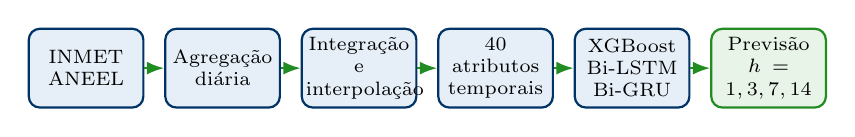
\begin{tikzpicture}[
    node distance=0.25cm,
    box/.style={
      rectangle, rounded corners, draw=UnBBlue, thick,
      fill=SoftBlue, text width=1.35cm, minimum height=1.0cm,
      inner sep=1.5pt, align=center, font=\scriptsize
    },
    final/.style={
      rectangle, rounded corners, draw=UnBGreen, thick,
      fill=SoftGreen, text width=1.35cm, minimum height=1.0cm,
      inner sep=1.5pt, align=center, font=\scriptsize
    },
    arrow/.style={-{Latex[length=2.2mm]}, thick, draw=UnBGreen}
  ]
    \node[box] (sources) {INMET\\ANEEL};
    \node[box, right=of sources] (daily) {Agregação\\diária};
    \node[box, right=of daily] (merge) {Integração e\\interpolação};
    \node[box, right=of merge] (features) {40 atributos\\temporais};
    \node[box, right=of features] (models) {XGBoost\\Bi-LSTM\\Bi-GRU};
    \node[final, right=of models] (forecast) {Previsão\\$h=1,3,7,14$};

    \draw[arrow] (sources) -- (daily);
    \draw[arrow] (daily) -- (merge);
    \draw[arrow] (merge) -- (features);
    \draw[arrow] (features) -- (models);
    \draw[arrow] (models) -- (forecast);
  \end{tikzpicture}

  \vspace{1.2em}
  \begin{itemize}
    \item Somatório para chuva e interrupções; médias para temperatura e vento.
    \item Interpolação linear apenas em lacunas curtas; extremos reais foram preservados.
    \item O consumo do SAMP foi integrado somente à análise exploratória mensal.
  \end{itemize}

  \source{Monografia, Seções 3.4 e 3.5.}
  \note{%
    Apresentador: Giovanni. Tempo-alvo: 1 minuto e 20 segundos.
    Percorrer o fluxo da esquerda para a direita. Explicar por que os outliers não foram removidos.
    [Sources] Monografia, Seções 3.4 e 3.5.
  }
\end{frame}

\begin{frame}{Atributos codificam memória e sazonalidade}{40 atributos derivados}
  \begin{columns}[T,onlytextwidth]
    \begin{column}{0.48\textwidth}
      \textbf{\large Memória recente}
      \begin{itemize}
        \item Defasagens de 1 a 7 dias.
        \item EMAs de 3, 7 e 14 dias.
        \item Desvio padrão móvel de 7 dias.
        \item Janela sequencial de 14 dias nas RNNs.
      \end{itemize}
    \end{column}
    \begin{column}{0.48\textwidth}
      \textbf{\large Contexto do sistema}
      \begin{itemize}
        \item Temperatura, chuva e cinco variáveis de vento.
        \item Histórico de interrupções disponível em $t$.
        \item Dia da semana e posição no ano.
        \item Codificação seno/cosseno do mês.
      \end{itemize}
    \end{column}
  \end{columns}

  \vspace{0.7em}
  \begin{block}{}
    As mesmas informações históricas disponíveis em $t$ alimentam a previsão direta de $t+h$.
  \end{block}

  \source{Monografia, Seções 3.4, 3.7 e 3.10.}
  \note{%
    Apresentador: Giovanni. Tempo-alvo: 1 minuto e 10 segundos.
    Distinguir features tabulares do lookback sequencial.
    [Sources] Monografia, Seções 3.4, 3.7, 3.9 e 3.10.
  }
\end{frame}

\begin{frame}{O teste preserva a ordem do tempo}{Protocolo sem vazamento de dados}
  \centering
  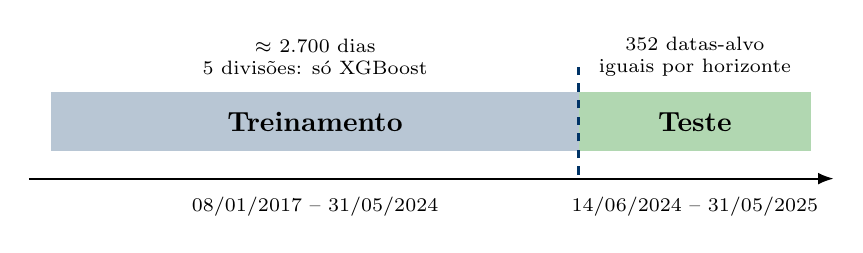
\begin{tikzpicture}[x=0.72cm,y=1cm]
    \draw[-{Latex[length=2mm]},thick] (0,0) -- (14.2,0);
    \fill[UnBBlue!28] (0.4,0.35) rectangle (9.7,1.1);
    \fill[UnBGreen!35] (9.7,0.35) rectangle (13.8,1.1);
    \draw[very thick,dashed,UnBBlue] (9.7,0.05) -- (9.7,1.45);
    \node at (5.05,0.72) {\textbf{Treinamento}};
    \node at (11.75,0.72) {\textbf{Teste}};
    \node[font=\scriptsize] at (5.05,-0.35) {08/01/2017 -- 31/05/2024};
    \node[font=\scriptsize] at (11.75,-0.35) {14/06/2024 -- 31/05/2025};
    \node[font=\scriptsize,align=center] at (5.05,1.55) {$\approx$ 2.700 dias\\5 divisões: só XGBoost};
    \node[font=\scriptsize,align=center] at (11.75,1.55) {352 datas-alvo\\iguais por horizonte};
  \end{tikzpicture}

  \vspace{1.2em}
  \begin{itemize}
    \item XGBoost: \texttt{TimeSeriesSplit} no treino; RNNs: 150 épocas fixas, sem validação interna.
    \item Normalização ajustada com dados até 31/05/2024.
    \item Modelos diretos independentes; nenhuma previsão intermediária é reutilizada.
  \end{itemize}

  \source{Monografia, Seções 3.6, 3.7 e 3.10.}
  \note{%
    Apresentador: Giovanni. Tempo-alvo: 1 minuto e 30 segundos.
    Este é o principal ponto de rigor metodológico: o futuro nunca entra no treino.
    [Sources] Monografia, Seções 3.6, 3.7 e 3.10.
  }
\end{frame}

\begin{frame}{Três modelos, três estratégias}{Arquiteturas comparadas}
  \begin{description}
    \item[XGBoost] Árvores sequenciais sobre atributos tabulares.\\
      \small 300 árvores, profundidade 4 e busca em grade com validação temporal.
    \item[Bi-LSTM] Memória recorrente com estado de célula.\\
      \small 2 camadas, 64 unidades, janela de 14 dias e dropout 0,4.
    \item[Bi-GRU] Memória recorrente mais compacta.\\
      \small 2 camadas, 64 unidades, janela de 14 dias e dropout 0,4.
  \end{description}

  \vspace{0.8em}
  \begin{block}{Comparação}
    MAE, RMSE, $R^2$ e MAPE sobre os mesmos 365 dias de teste.
  \end{block}

  \source{Monografia, Seção 3.9.}
  \note{%
    Apresentador: Giovanni. Tempo-alvo: 1 minuto e 20 segundos.
    Explicar a diferença entre engenharia explícita do XGBoost e memória aprendida pelas RNNs.
    [Sources] Monografia, Seção 3.9.
  }
\end{frame}

\section{Resultados exploratórios}

\begin{frame}{A série revela tendência e sazonalidade}{2017--2025}
  \centering
  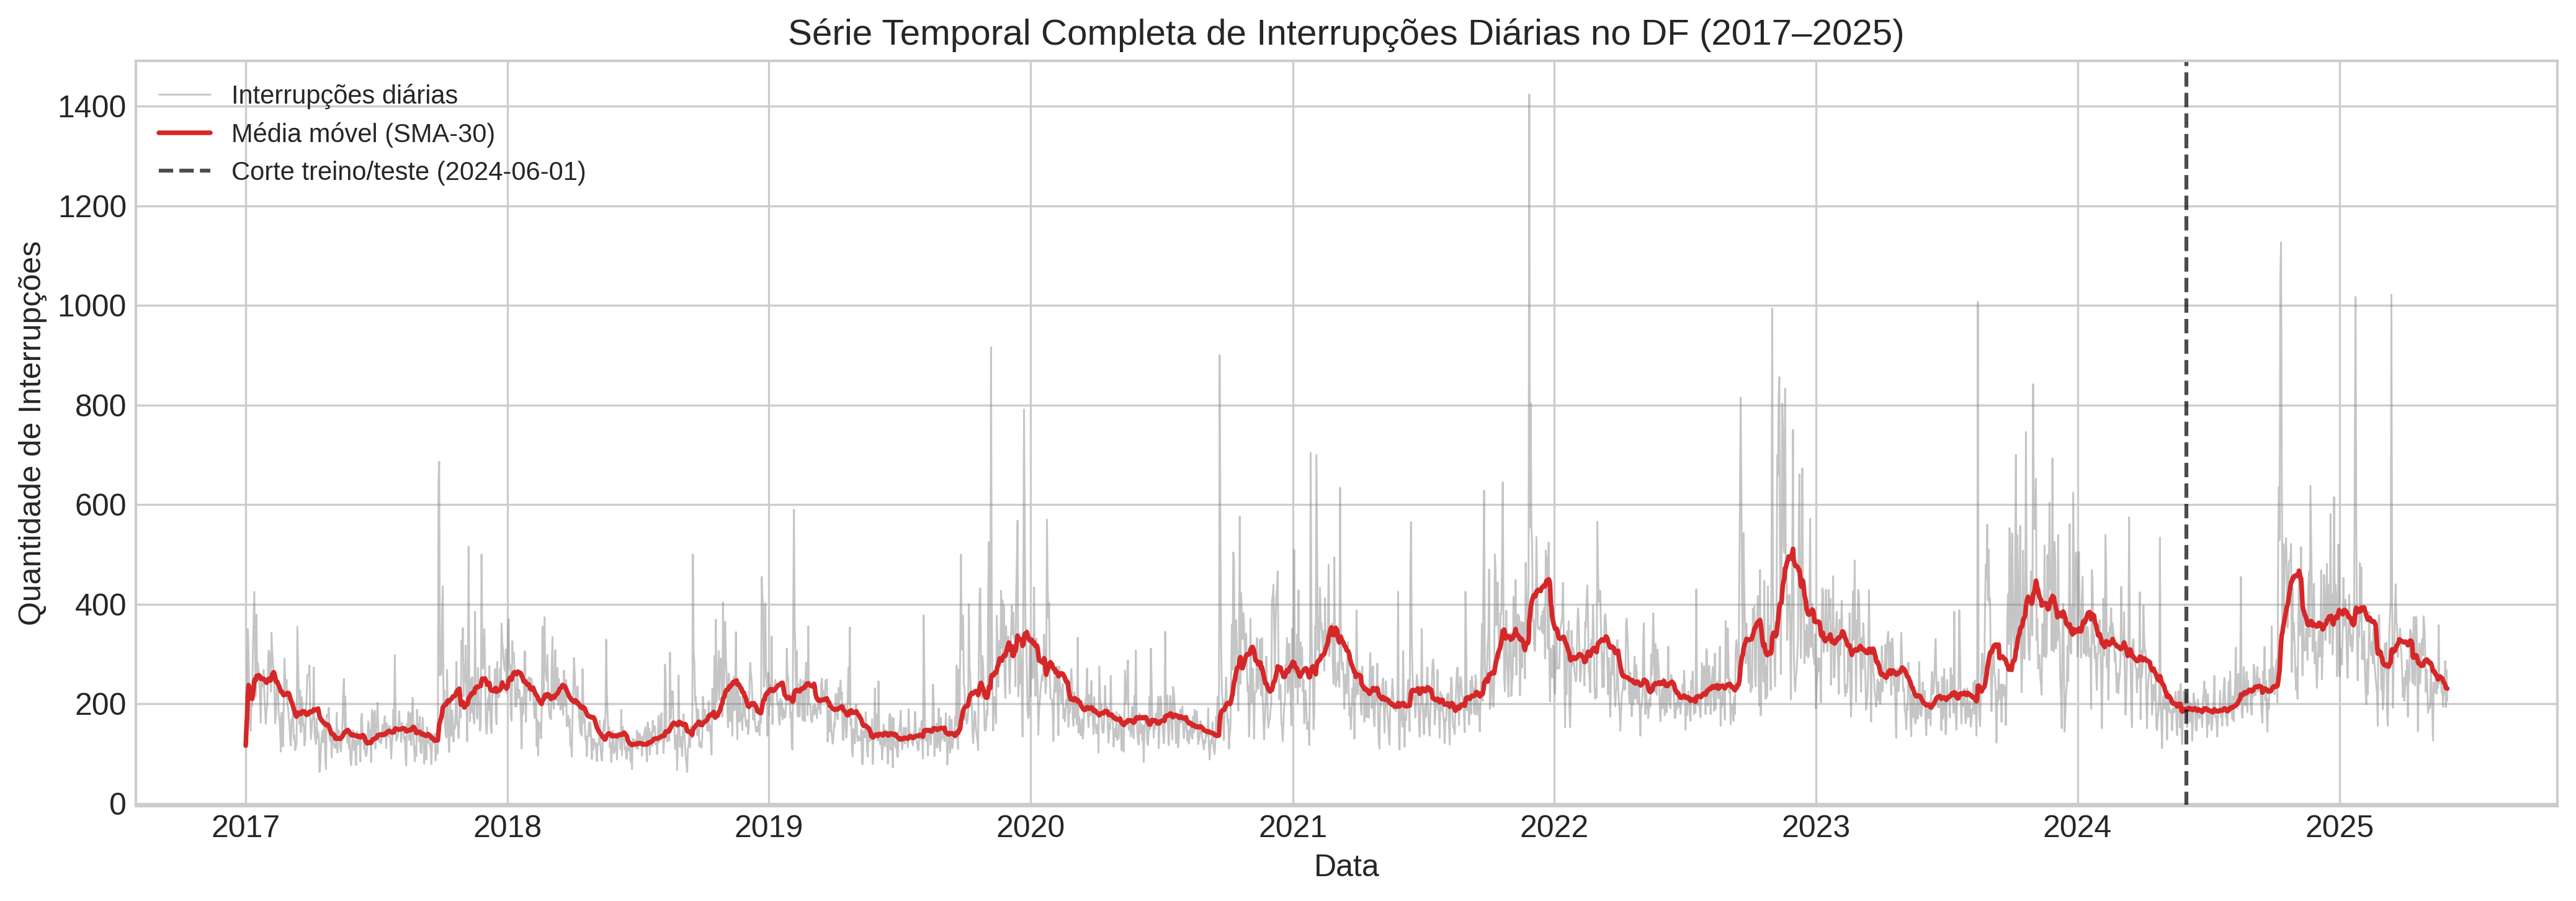
\includegraphics[width=0.98\textwidth]{serie_temporal_completa.png}

  \vspace{-0.2em}
  \begin{itemize}
    \item Picos recorrentes entre outubro e março.
    \item Vale operacional predominante entre maio e agosto.
    \item Eventos acima de 1.000 interrupções permanecem raros.
  \end{itemize}

  \source{ANEEL; elaboração dos autores, Figura 4.1.}
  \note{%
    Apresentador: Giovanni. Tempo-alvo: 1 minuto e 20 segundos.
    Encerrar a primeira parte mostrando a estrutura visual da série.
    [Sources] Monografia, Seção 4.1 e Figura 4.1.
  }
\end{frame}

% ------------------------------------------------------------------
% RESULTADOS E CONCLUSÃO — Mateus
% ------------------------------------------------------------------

\begin{frame}{A série mantém memória além de 14 dias}{Autocorrelação}
  \centering
  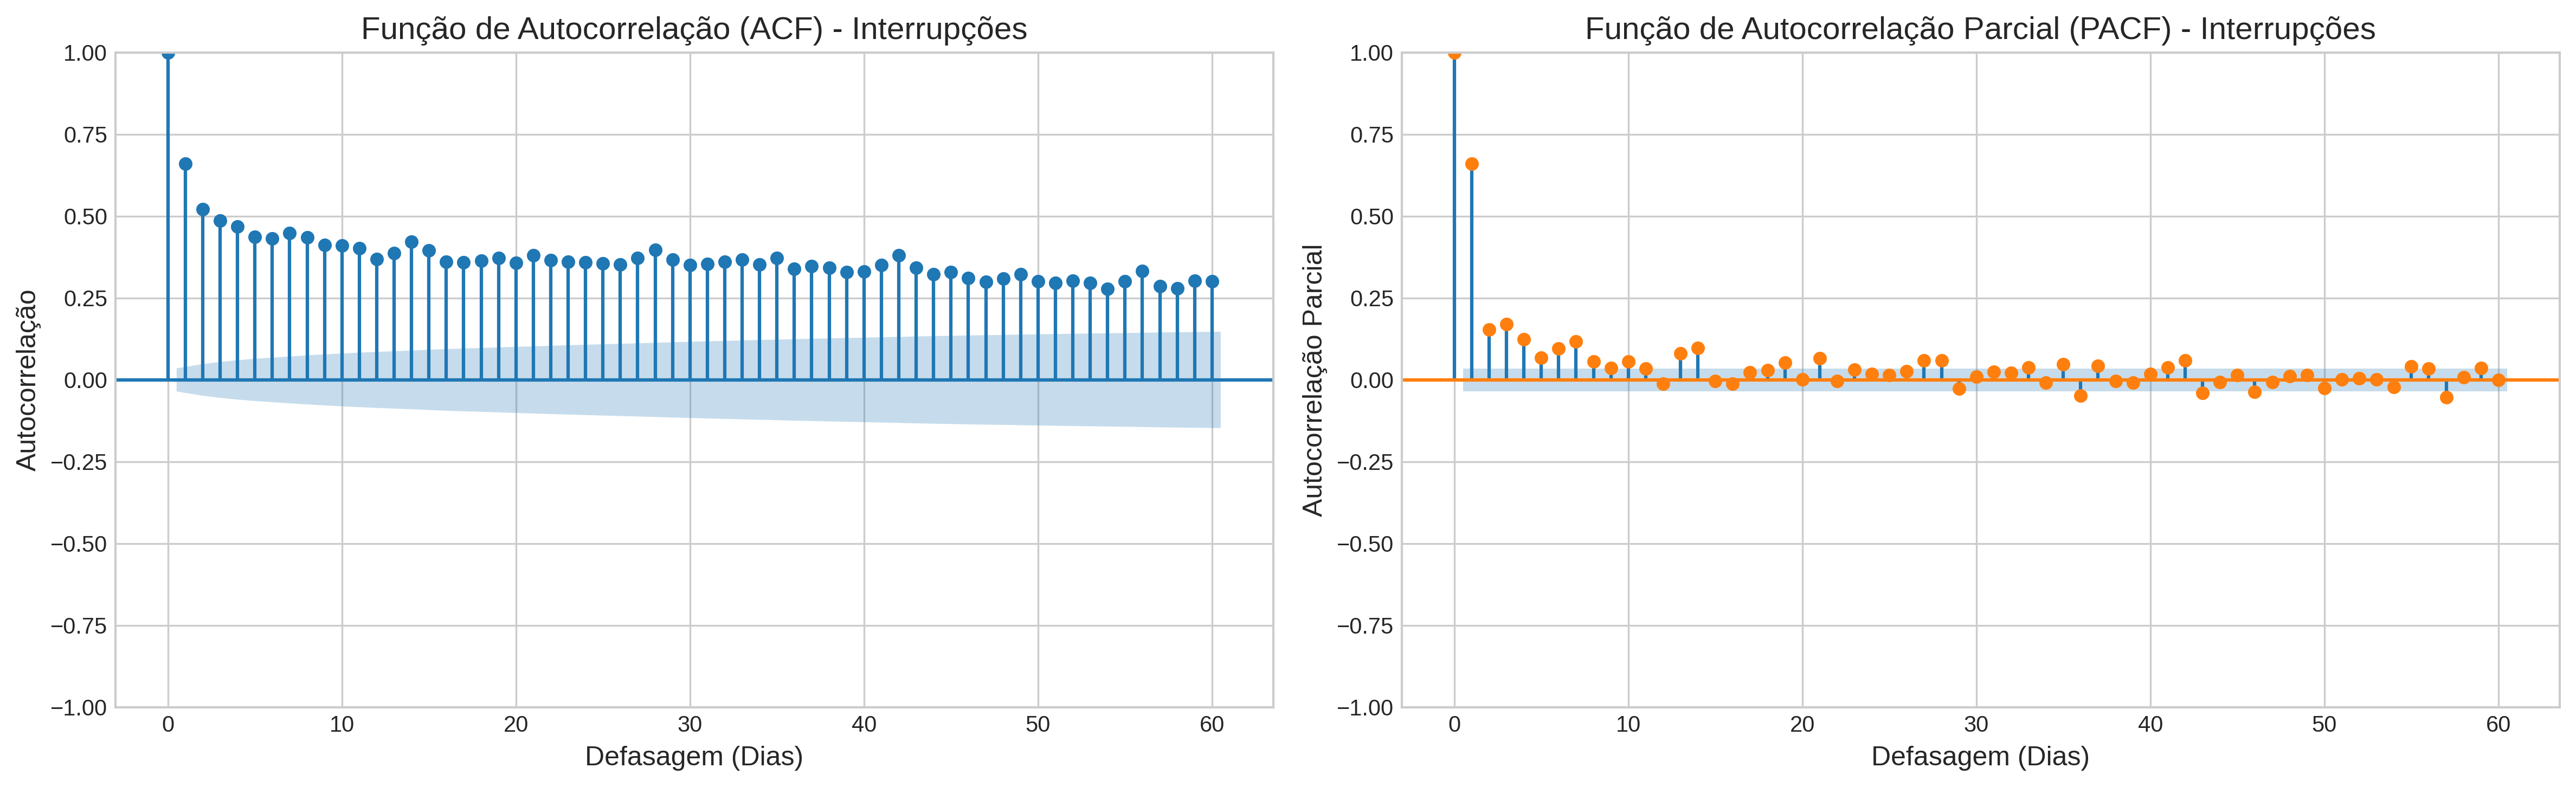
\includegraphics[width=0.96\textwidth]{autocorrelacao_interrupcoes.png}

  \vspace{-0.2em}
  \begin{block}{Leitura}
    A dependência temporal significativa fundamenta lags, EMAs e a janela recorrente de 14 dias.
  \end{block}

  \source{Elaboração dos autores, Figura 4.5.}
  \note{%
    Apresentador: Mateus. Tempo-alvo: 1 minuto e 15 segundos.
    Assumir a fala a partir daqui. Mostrar o decaimento da ACF e a evidência para o lookback.
    [Sources] Monografia, Seção 4.2 e Figura 4.5.
  }
\end{frame}

\begin{frame}{A agregação revela melhor o sinal climático}{Correlação com interrupções}
  \begin{columns}[T,onlytextwidth]
    \begin{column}{0.70\textwidth}
      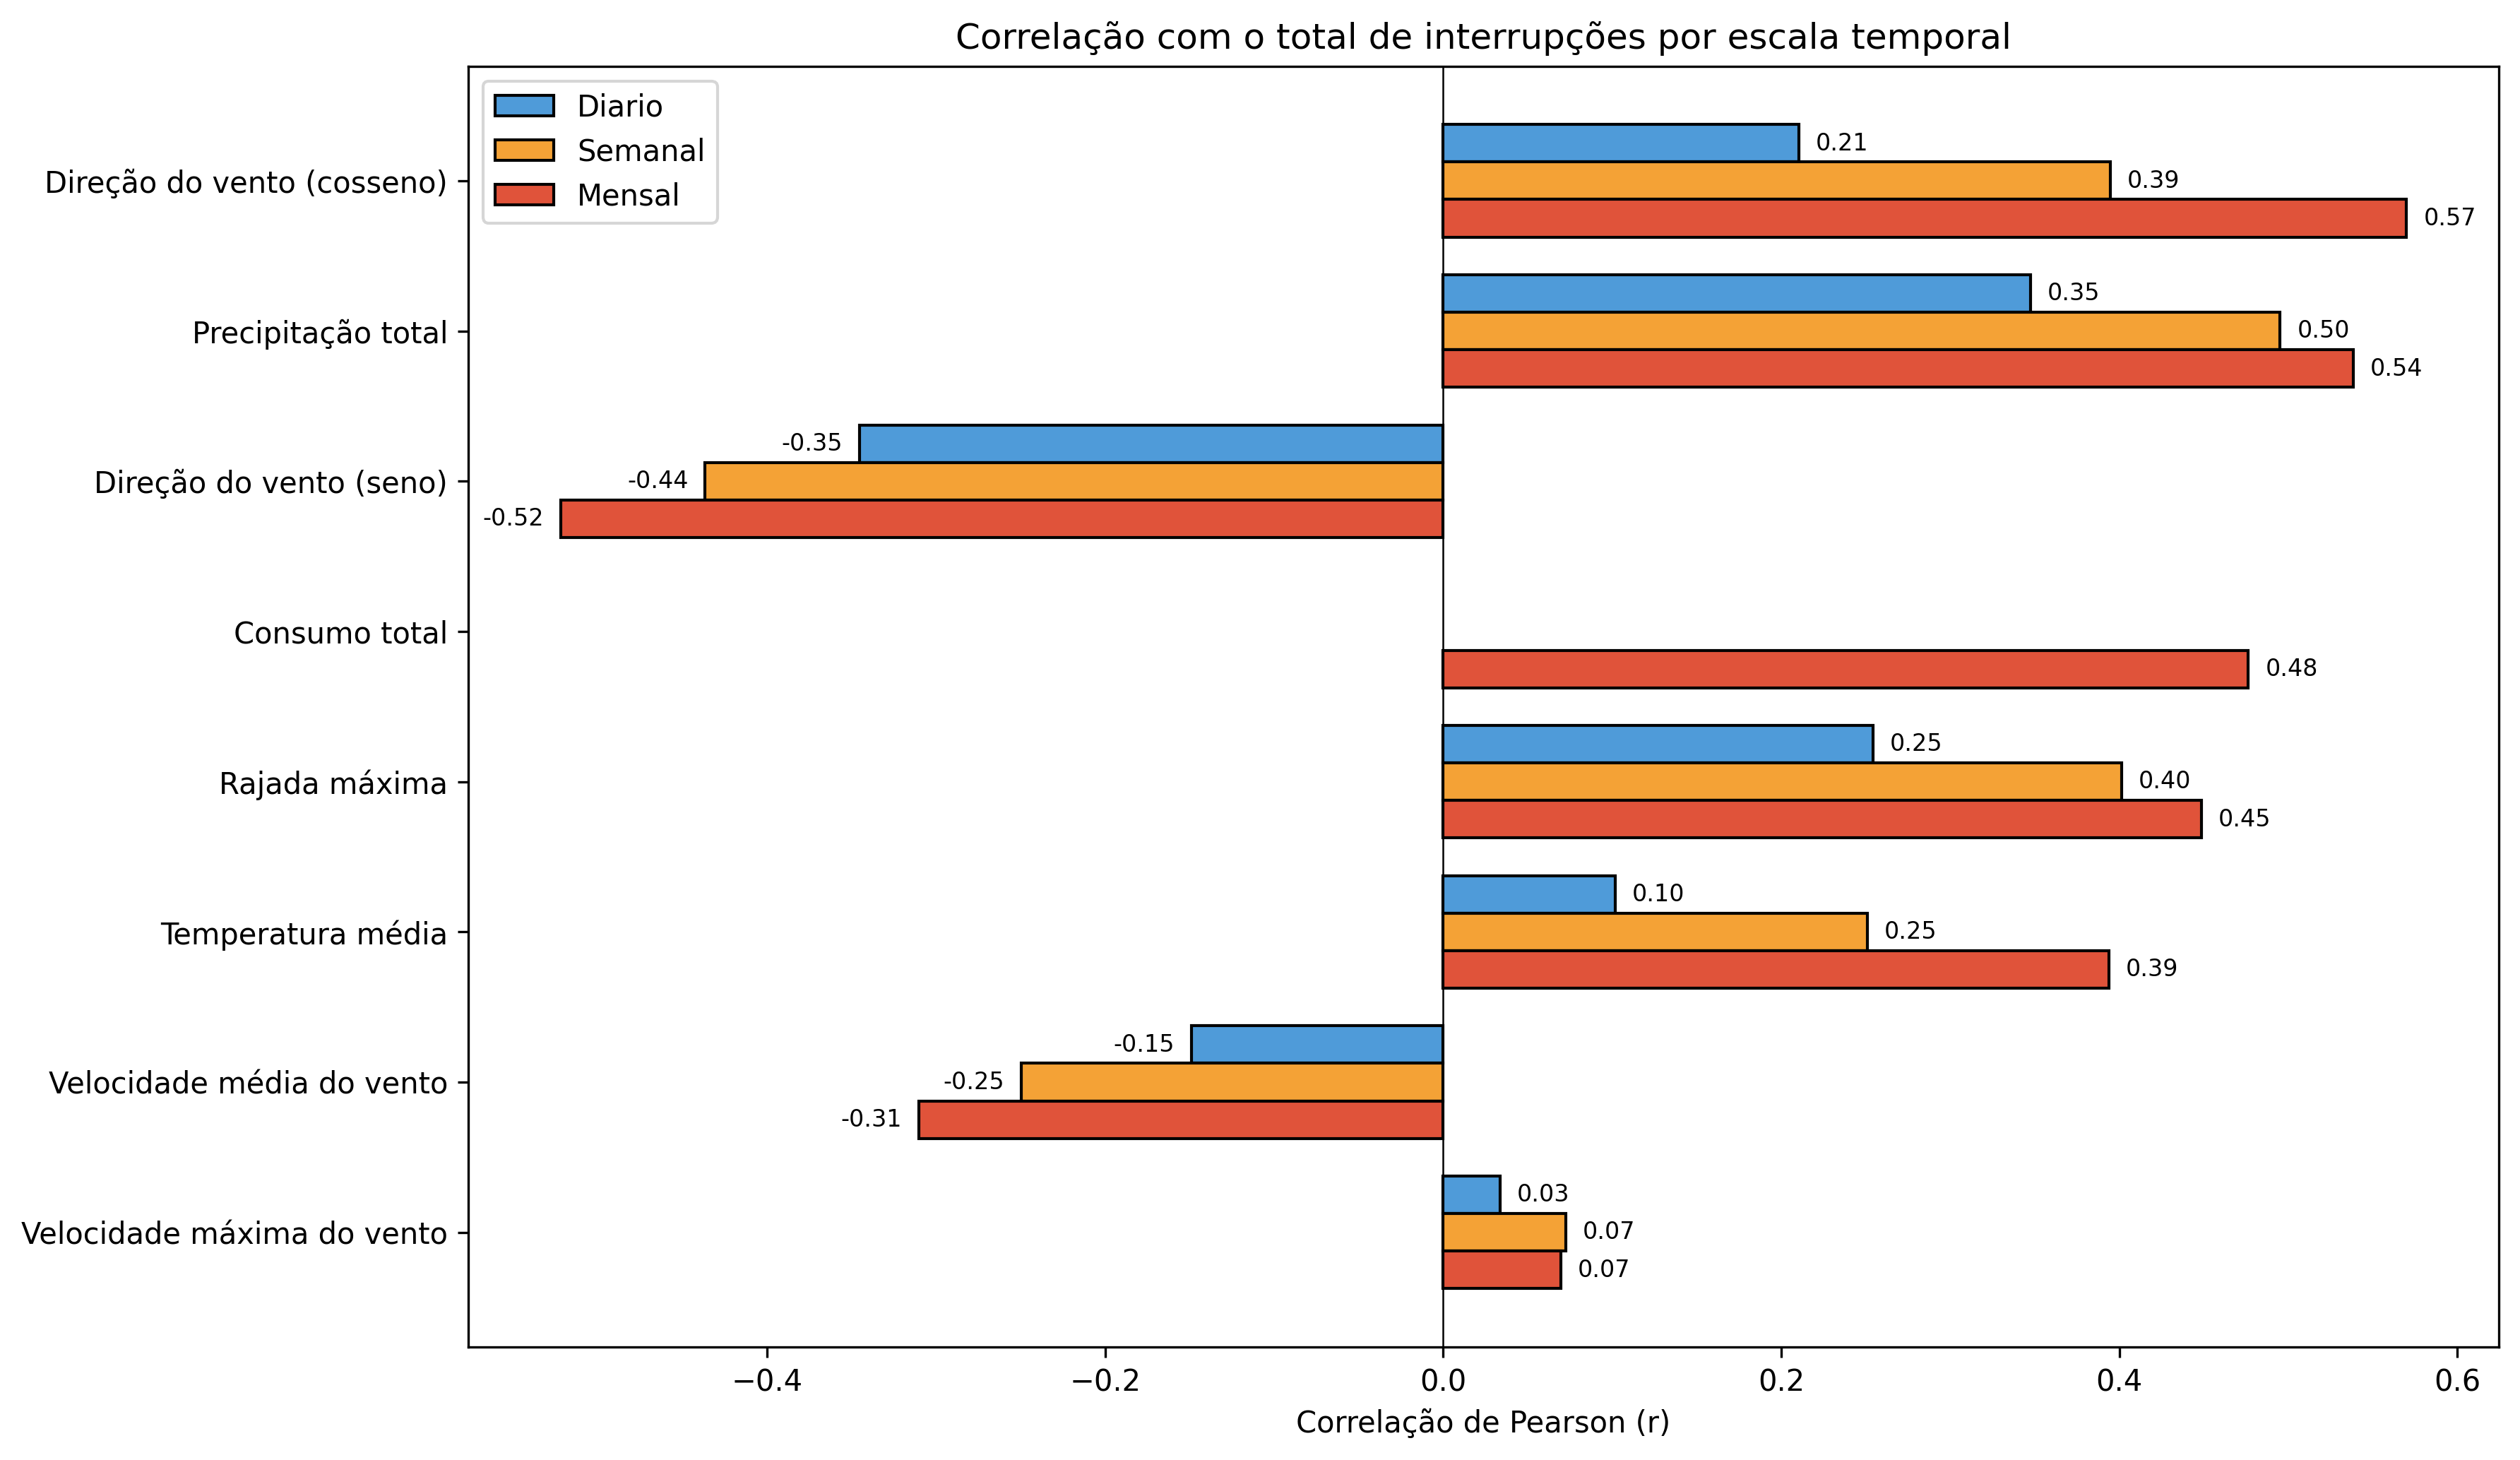
\includegraphics[width=\textwidth]{correlacoes_escala_temporal.png}
    \end{column}
    \begin{column}{0.27\textwidth}
      \vspace{0.6em}
      \keynumber{0,59}{direção do vento, mensal}
      \vspace{0.9em}
      \keynumber{0,54}{precipitação, mensal}
      \vspace{0.9em}
      \keynumber{0,48}{consumo, mensal\\{\scriptsize (exploratório)}}
    \end{column}
  \end{columns}

  \source{INMET e ANEEL; elaboração dos autores, Figura 4.8.}
  \note{%
    Apresentador: Mateus. Tempo-alvo: 1 minuto e 30 segundos.
    Explicar que agregação reduz ruído e capta efeitos cumulativos. Reforçar que correlação não prova causalidade.
    [Sources] Monografia, Seção 4.3 e Tabela 4.1.
  }
\end{frame}

\section{Desempenho preditivo}

\begin{frame}{XGBoost e Bi-LSTM têm MAE próximo}{Resultados para $h=1$}
  \begin{columns}[T,onlytextwidth]
    \begin{column}{0.62\textwidth}
      \resizebox{\linewidth}{!}{%
        \begin{tabular}{lrrrr}
          \toprule
          \textbf{Modelo} & \textbf{MAE} & \textbf{RMSE} & \textbf{$R^2$} & \textbf{MAPE} \\
          \midrule
          \textbf{XGBoost} & \textbf{61,09} & 99,72 & 0,409 & \textbf{20,64\%} \\
          \textbf{Bi-LSTM} & 62,71 & \textbf{98,80} & \textbf{0,420} & 20,94\% \\
          Bi-GRU & 73,44 & 119,21 & 0,156 & 26,18\% \\
          \bottomrule
        \end{tabular}%
      }
    \end{column}
    \begin{column}{0.34\textwidth}
      \vspace{0.2em}
      \keynumber{2,7\%}{diferença de MAE entre XGBoost e Bi-LSTM}
      \vspace{1.0em}
      \textbf{Interpretação}\\
      Com as mesmas 40 \textit{features}, XGBoost e Bi-LSTM tiveram desempenho próximo em $h=1$.
    \end{column}
  \end{columns}

  \source{Elaboração dos autores; 365 dias de teste.}
  \note{%
    Apresentador: Mateus. Tempo-alvo: 1 minuto e 30 segundos.
    Evitar declarar vencedor absoluto: XGBoost vence em MAE/MAPE; Bi-LSTM em RMSE e R2. Ambos recebem as mesmas features engenheiradas.
    [Sources] Monografia, Tabela 4.2; arquivos de métricas do repositório.
  }
\end{frame}

\begin{frame}{Os modelos suavizam os maiores picos}{XGBoost no conjunto de teste}
  \centering
  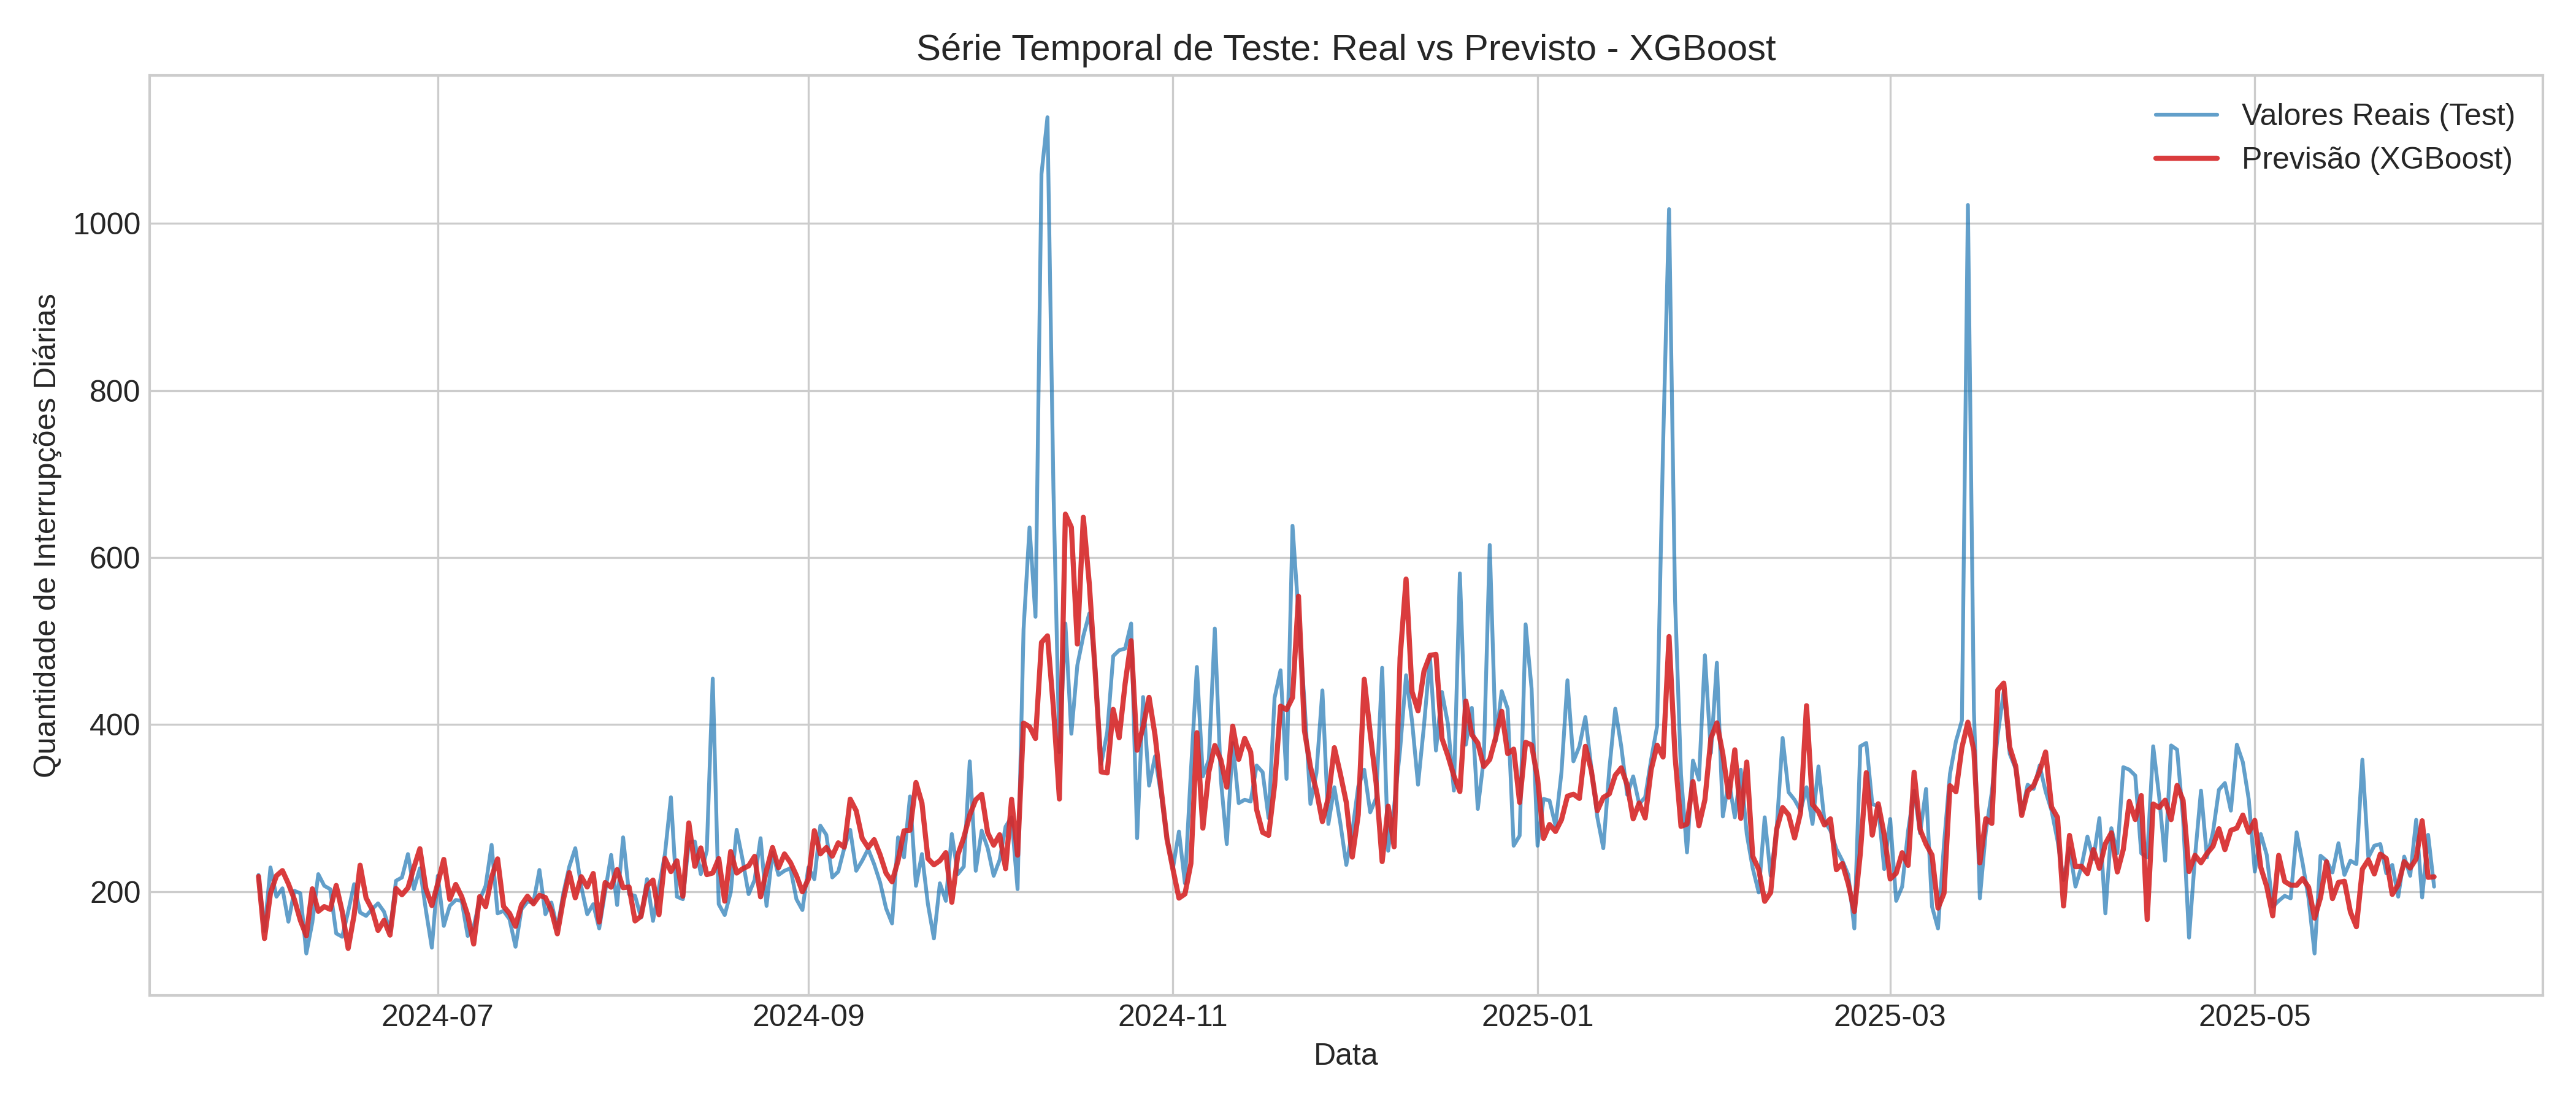
\includegraphics[width=0.98\textwidth]{ts_pred_xgboost.png}

  \vspace{-0.2em}
  \begin{block}{}
    O desempenho médio é útil, mas os maiores eventos ainda são sistematicamente subestimados.
  \end{block}

  \source{Elaboração dos autores, Figura 4.20.}
  \note{%
    Apresentador: Mateus. Tempo-alvo: 1 minuto e 10 segundos.
    Apontar os picos de outubro, janeiro e março e a compressão para a média.
    [Sources] Monografia, Seção 4.4.2 e Figura 4.20.
  }
\end{frame}

\begin{frame}{O erro cresce nos dias mais críticos}{Heteroscedasticidade e severidade}
  \begin{columns}[T,onlytextwidth]
    \begin{column}{0.57\textwidth}
      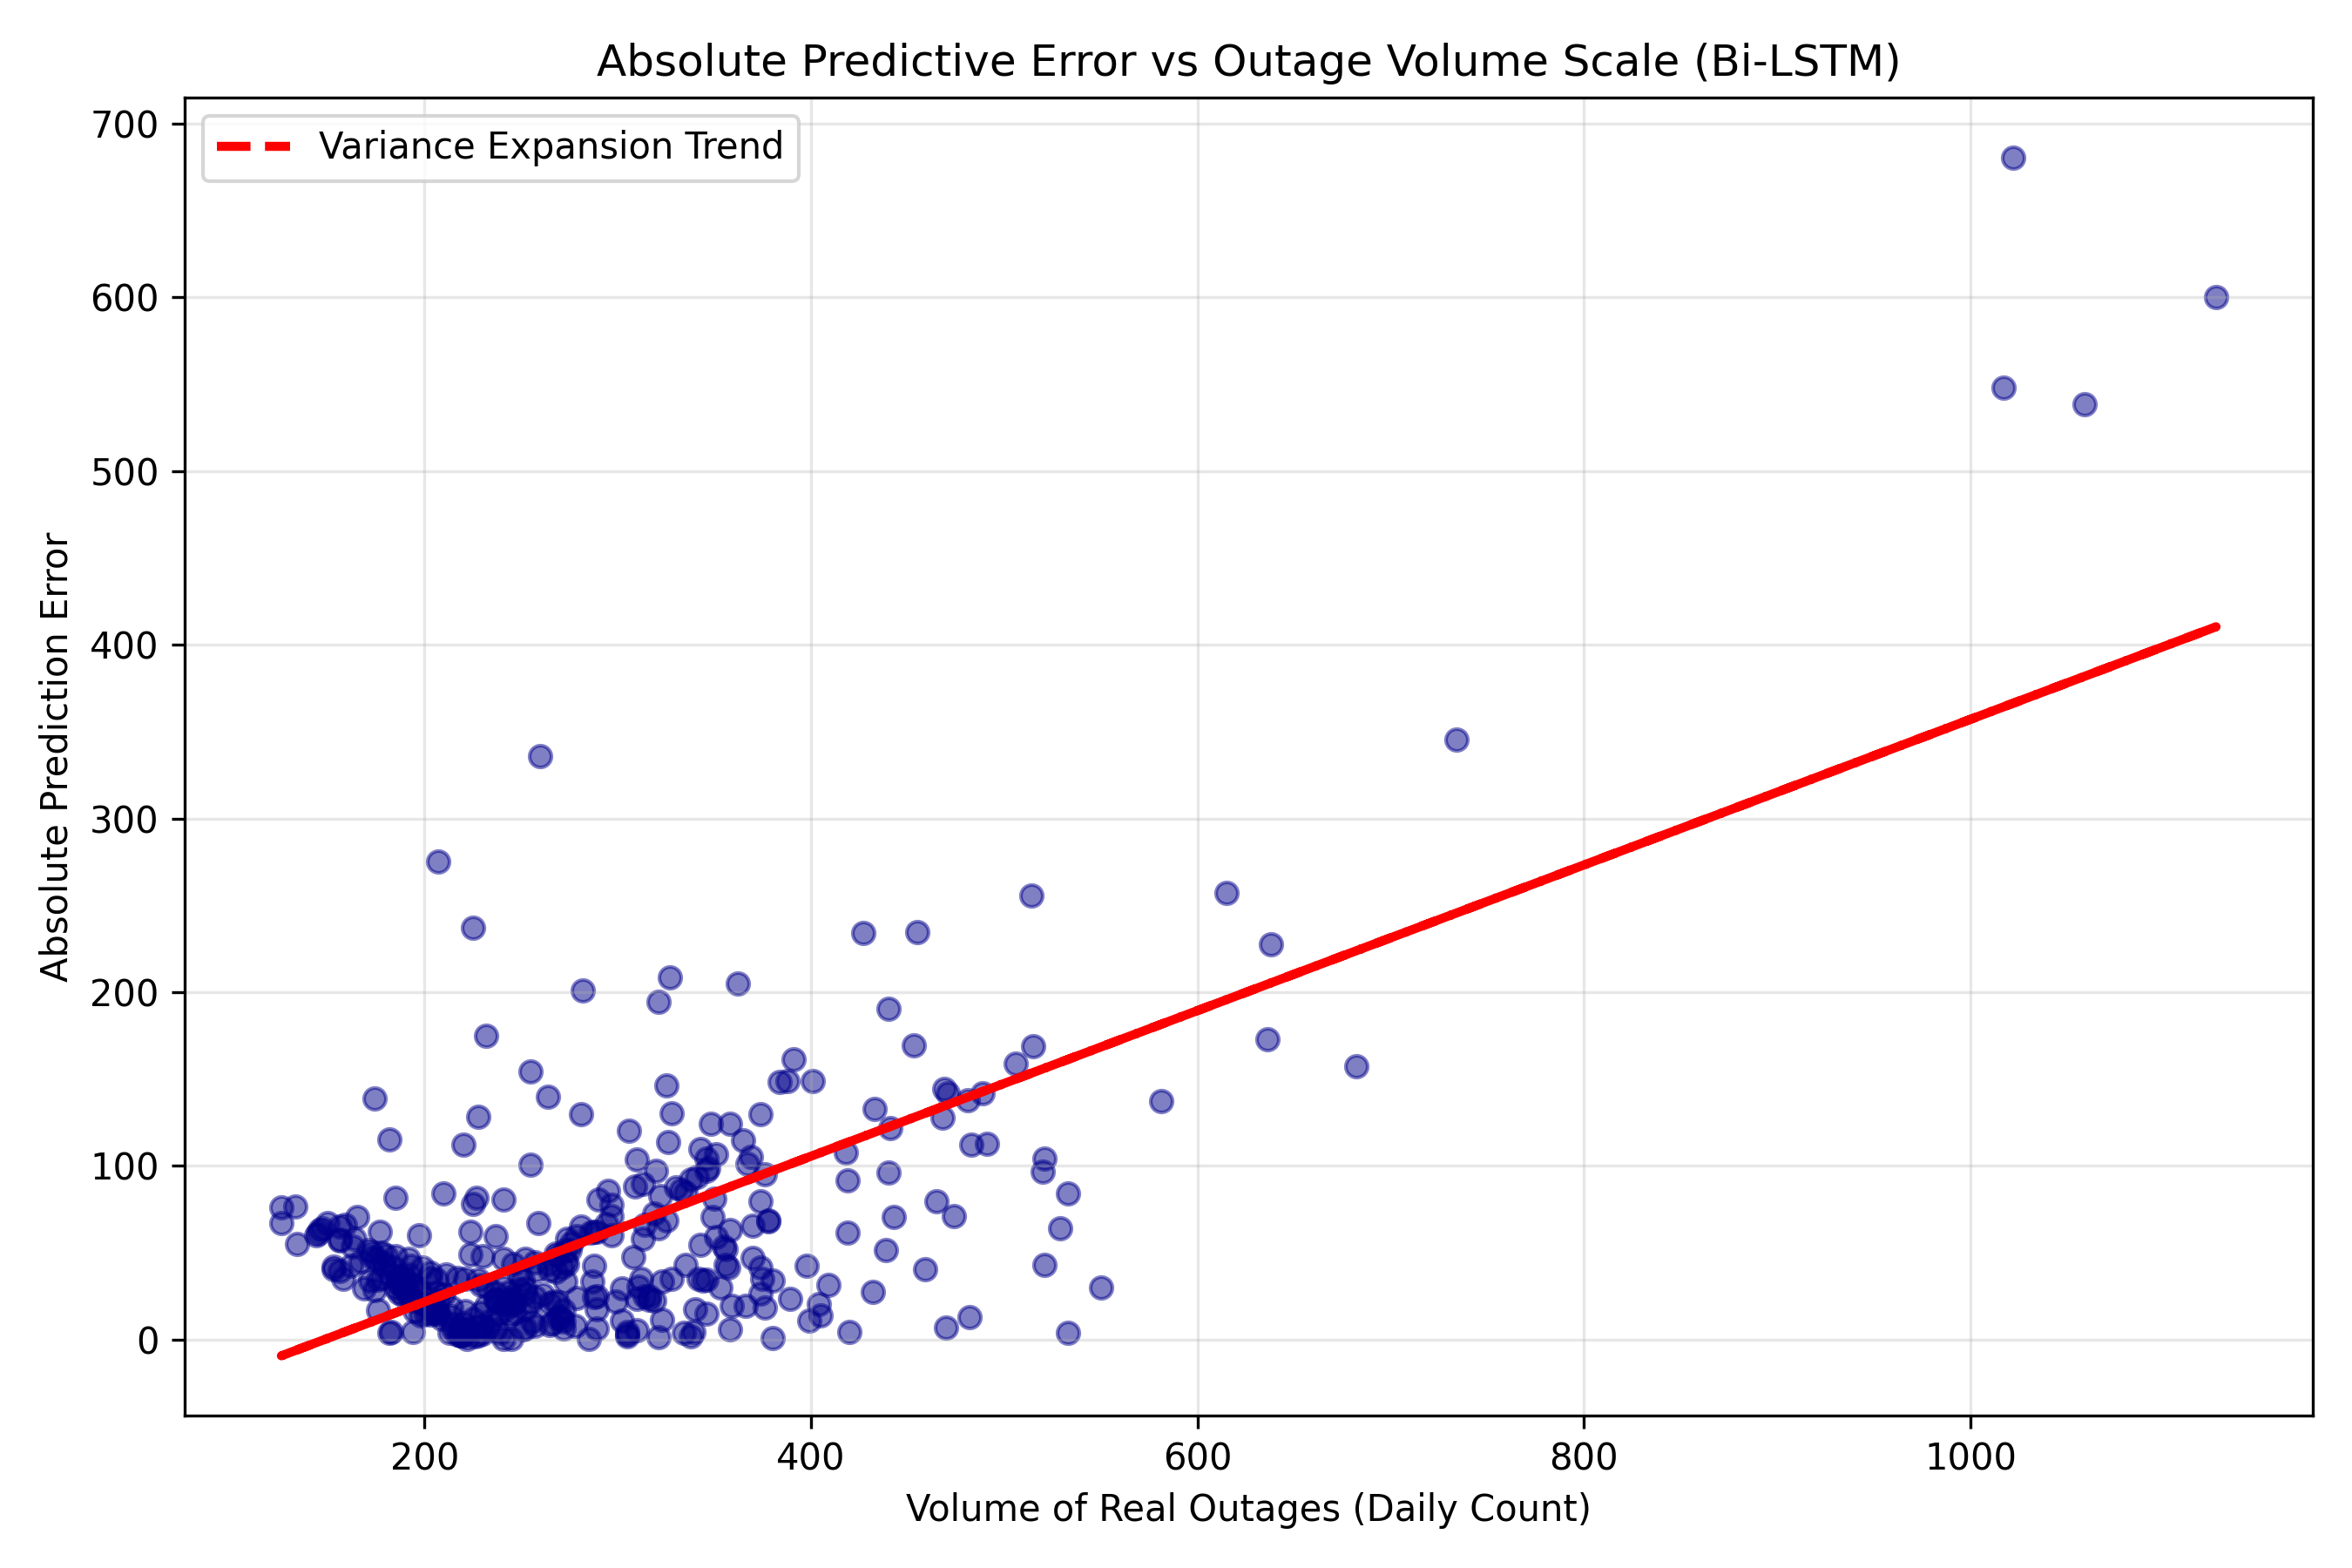
\includegraphics[width=\textwidth]{scatter_heteroscedasticity.png}
    \end{column}
    \begin{column}{0.39\textwidth}
      \textbf{\large MAE do XGBoost}
      \vspace{0.6em}

      \modelwinner{Normal ($<200$)}{30,1}{20,3\% dos dias}
      \modelwinner{Moderada (200--400)}{38,9}{66,0\% dos dias}
      \modelwinner{Severa ($>400$)}{135,9}{13,7\% dos dias}

      \vspace{0.6em}
      \small
      Previsões pontuais devem evoluir para intervalos de incerteza.
    \end{column}
  \end{columns}

  \source{Elaboração dos autores, Tabela 4.3 e Figura 4.27.}
  \note{%
    Apresentador: Mateus. Tempo-alvo: 1 minuto e 20 segundos.
    Destacar que o erro quadruplica nos dias severos, exatamente os mais importantes operacionalmente.
    [Sources] Monografia, Seções 4.4.4 e 4.5.
  }
\end{frame}

\begin{frame}{O histórico domina o curto prazo}{Importância no XGBoost}
  \begin{columns}[T,onlytextwidth]
    \begin{column}{0.69\textwidth}
      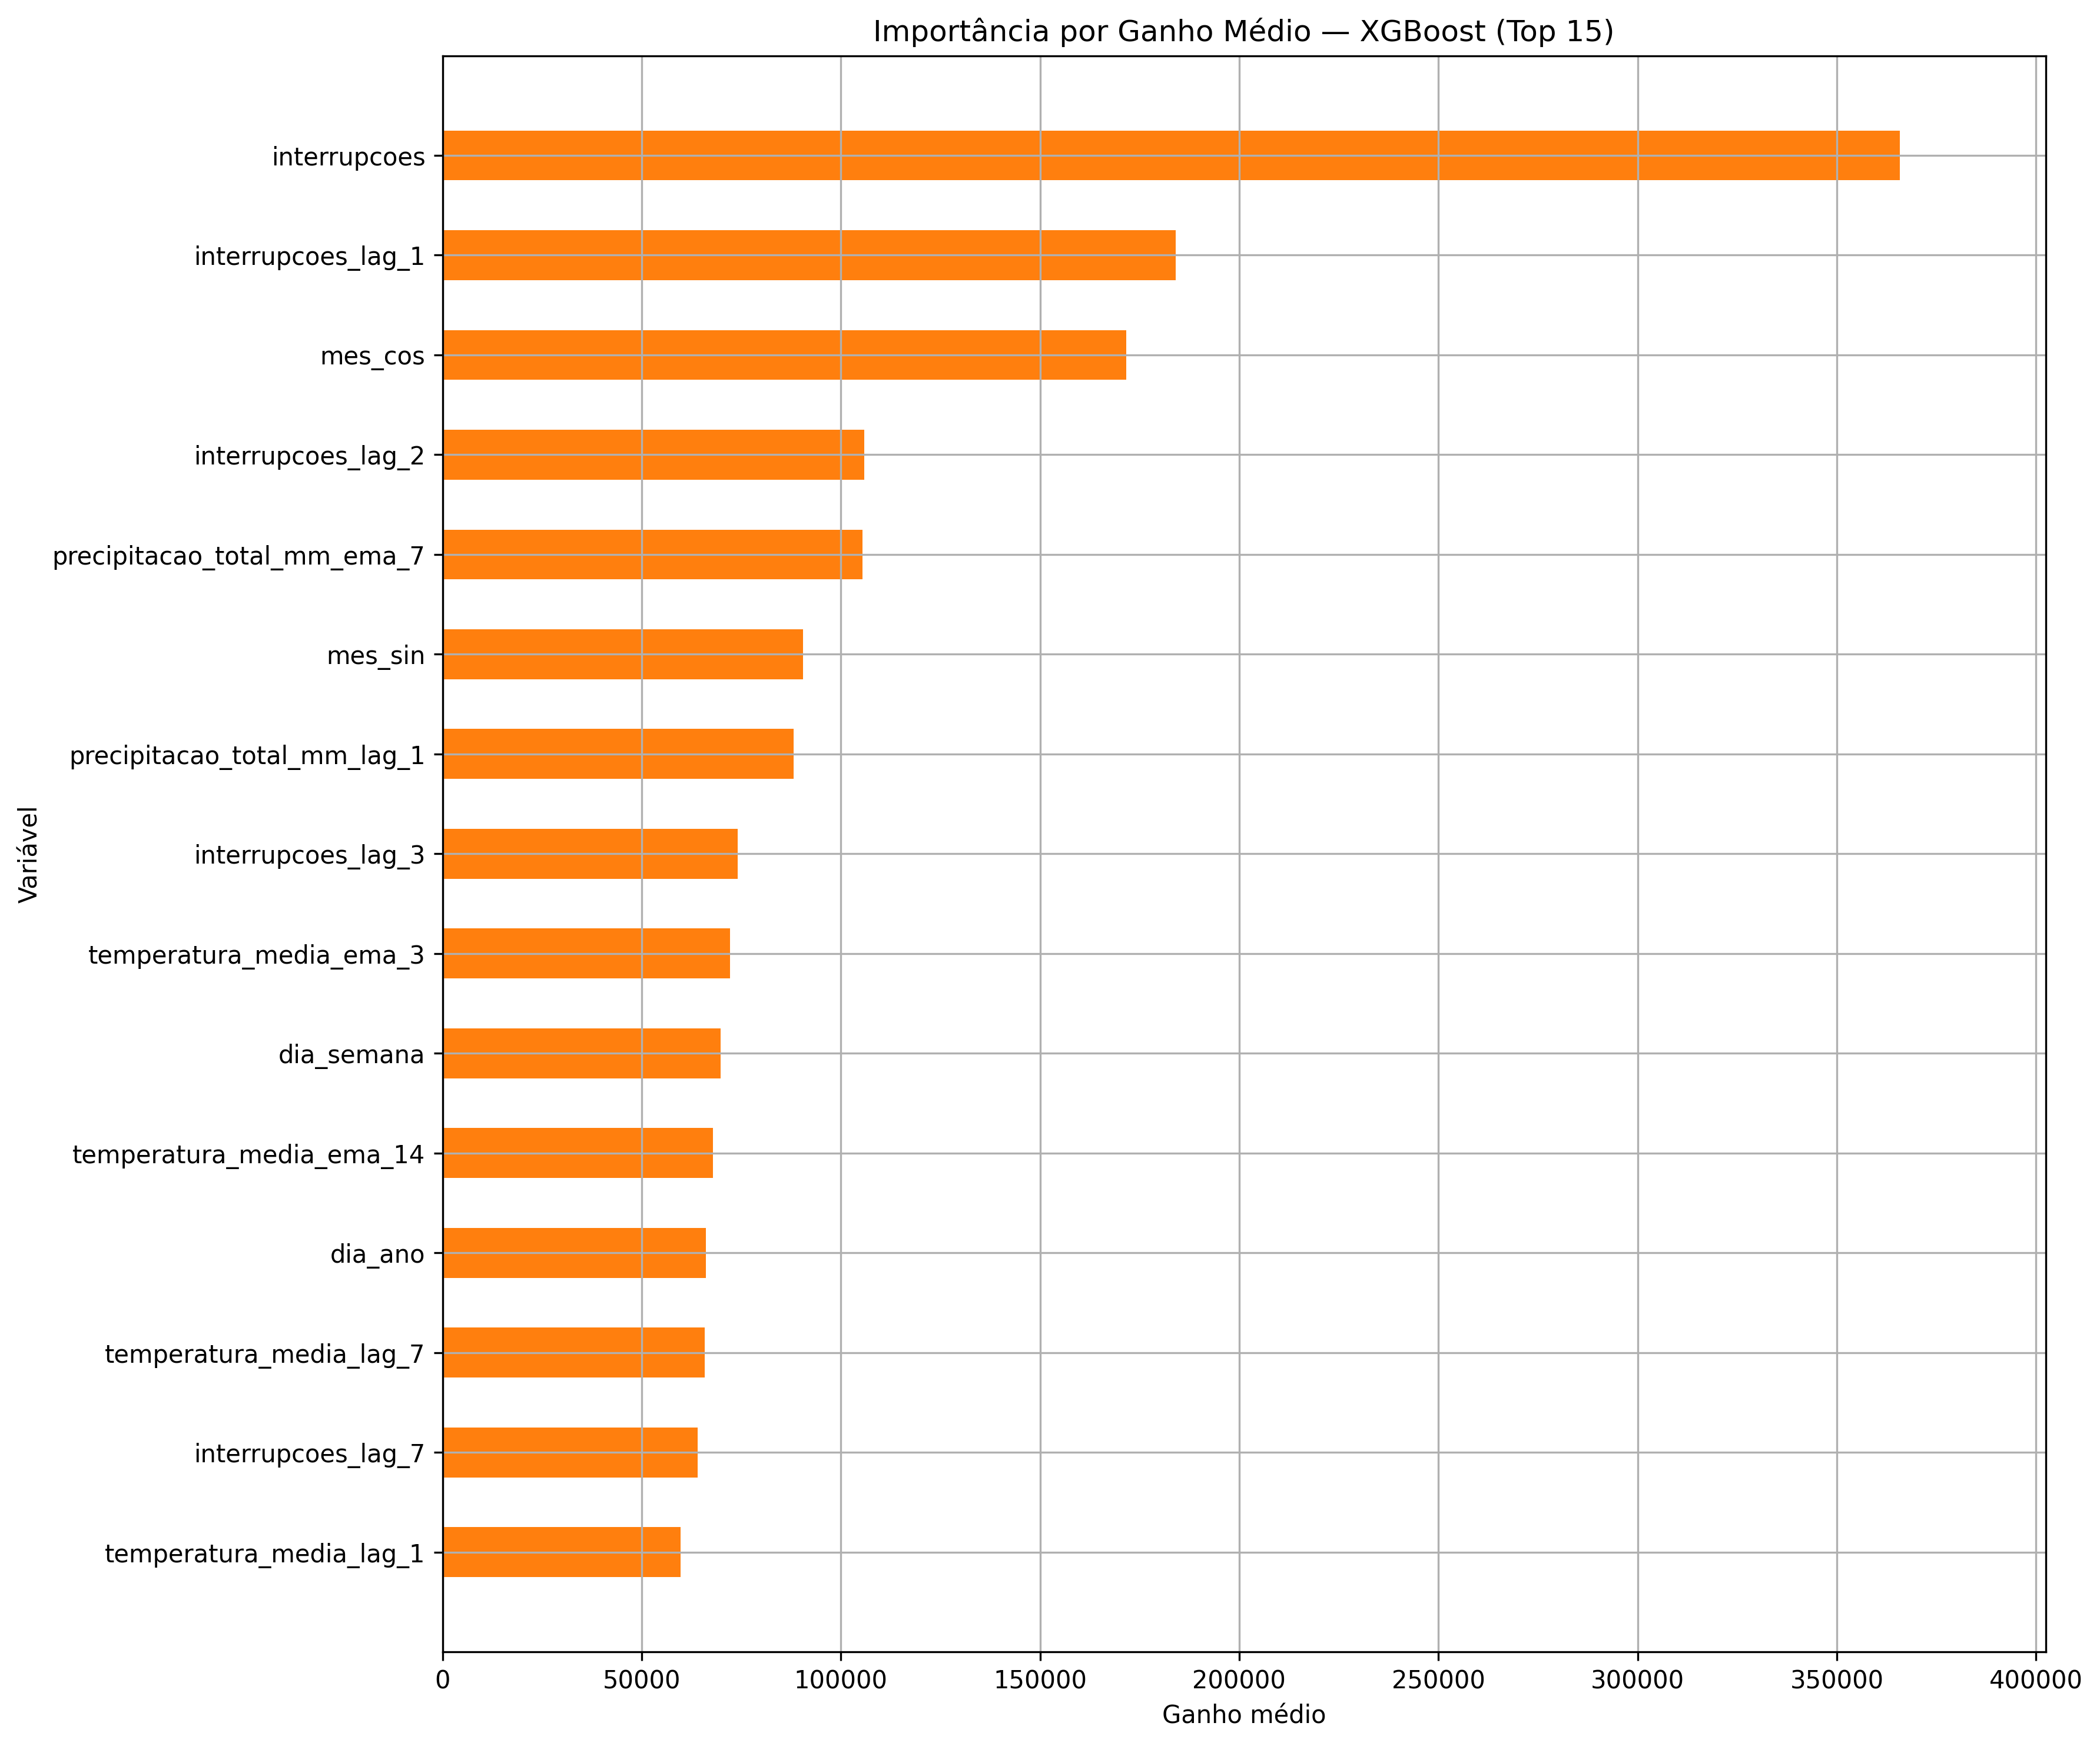
\includegraphics[width=\textwidth]{feature_importance_xgboost.png}
    \end{column}
    \begin{column}{0.28\textwidth}
      \textbf{\large Principais sinais}
      \begin{itemize}
        \item Interrupções em $t$.
        \item Lag de 1 dia.
        \item Sazonalidade mensal.
        \item EMA de precipitação.
      \end{itemize}

      \small
      Importância preditiva não implica causalidade.
    \end{column}
  \end{columns}

  \source{Elaboração dos autores, Figura 4.29.}
  \note{%
    Apresentador: Mateus. Tempo-alvo: 1 minuto e 15 segundos.
    Mostrar como o estado recente da rede, a estação do ano e a chuva acumulada formam a previsão.
    [Sources] Monografia, Seção 4.8 e Figura 4.29.
  }
\end{frame}

\begin{frame}{A hierarquia muda com o horizonte}{MAE em previsão direta}
  \begin{columns}[T,onlytextwidth]
    \begin{column}{0.72\textwidth}
      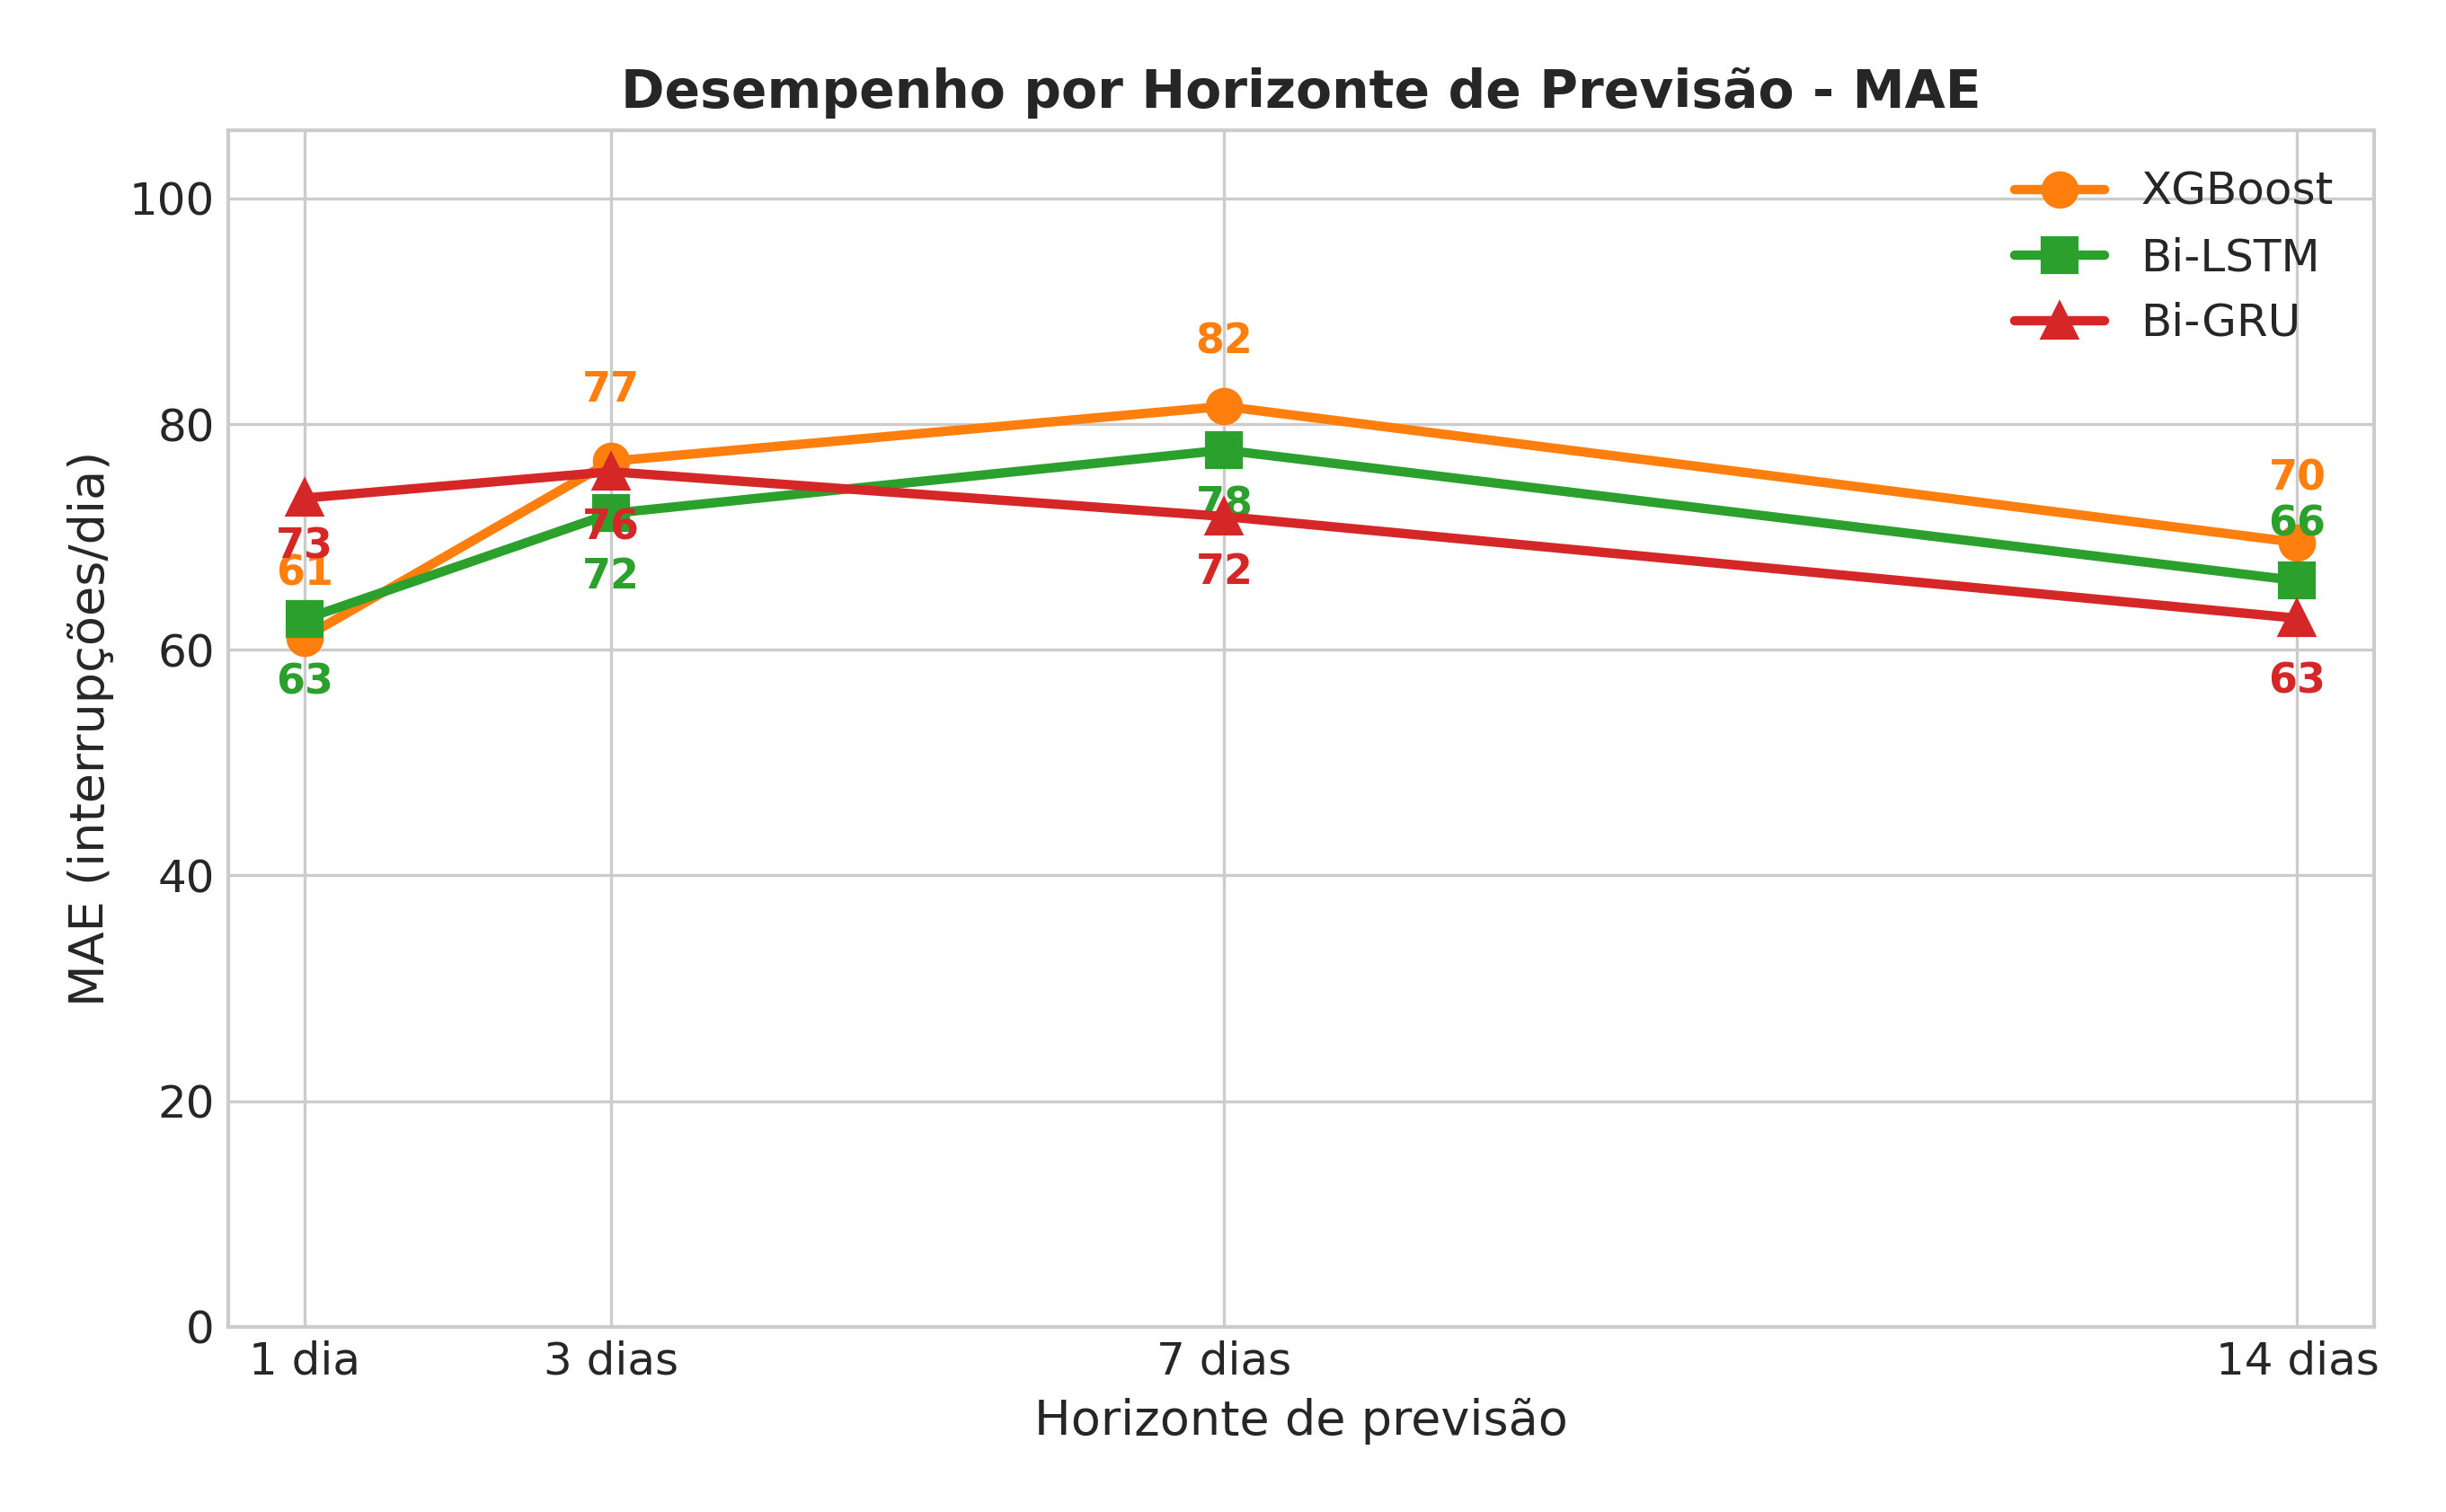
\includegraphics[width=\textwidth]{previsao_multihorizonte_degradacao.png}
    \end{column}
    \begin{column}{0.25\textwidth}
      \vspace{0.4em}
      \modelwinner{$h=1$}{XGBoost}{MAE 62,5}
      \modelwinner{$h=3$}{Bi-LSTM}{MAE 74,0}
      \modelwinner{$h=7$}{Bi-GRU}{MAE 73,6}
      \modelwinner{$h=14$}{Bi-GRU}{MAE 64,3}
    \end{column}
  \end{columns}

  \source{Elaboração dos autores; 352 alvos causais; XGBoost reutiliza os hiperparâmetros de $h=1$.}
  \note{%
    Apresentador: Mateus. Tempo-alvo: 1 minuto e 40 segundos.
    Este é o principal resultado comparativo. Explicar que cada ponto vem de um modelo treinado diretamente para aquele horizonte.
    [Sources] Monografia, Seção 4.10 e Figura 4.34; arquivo de métricas multi-horizonte.
  }
\end{frame}

\begin{frame}{Erros aumentam na transição chuvosa}{Variação mensal do MAE}
  \centering
  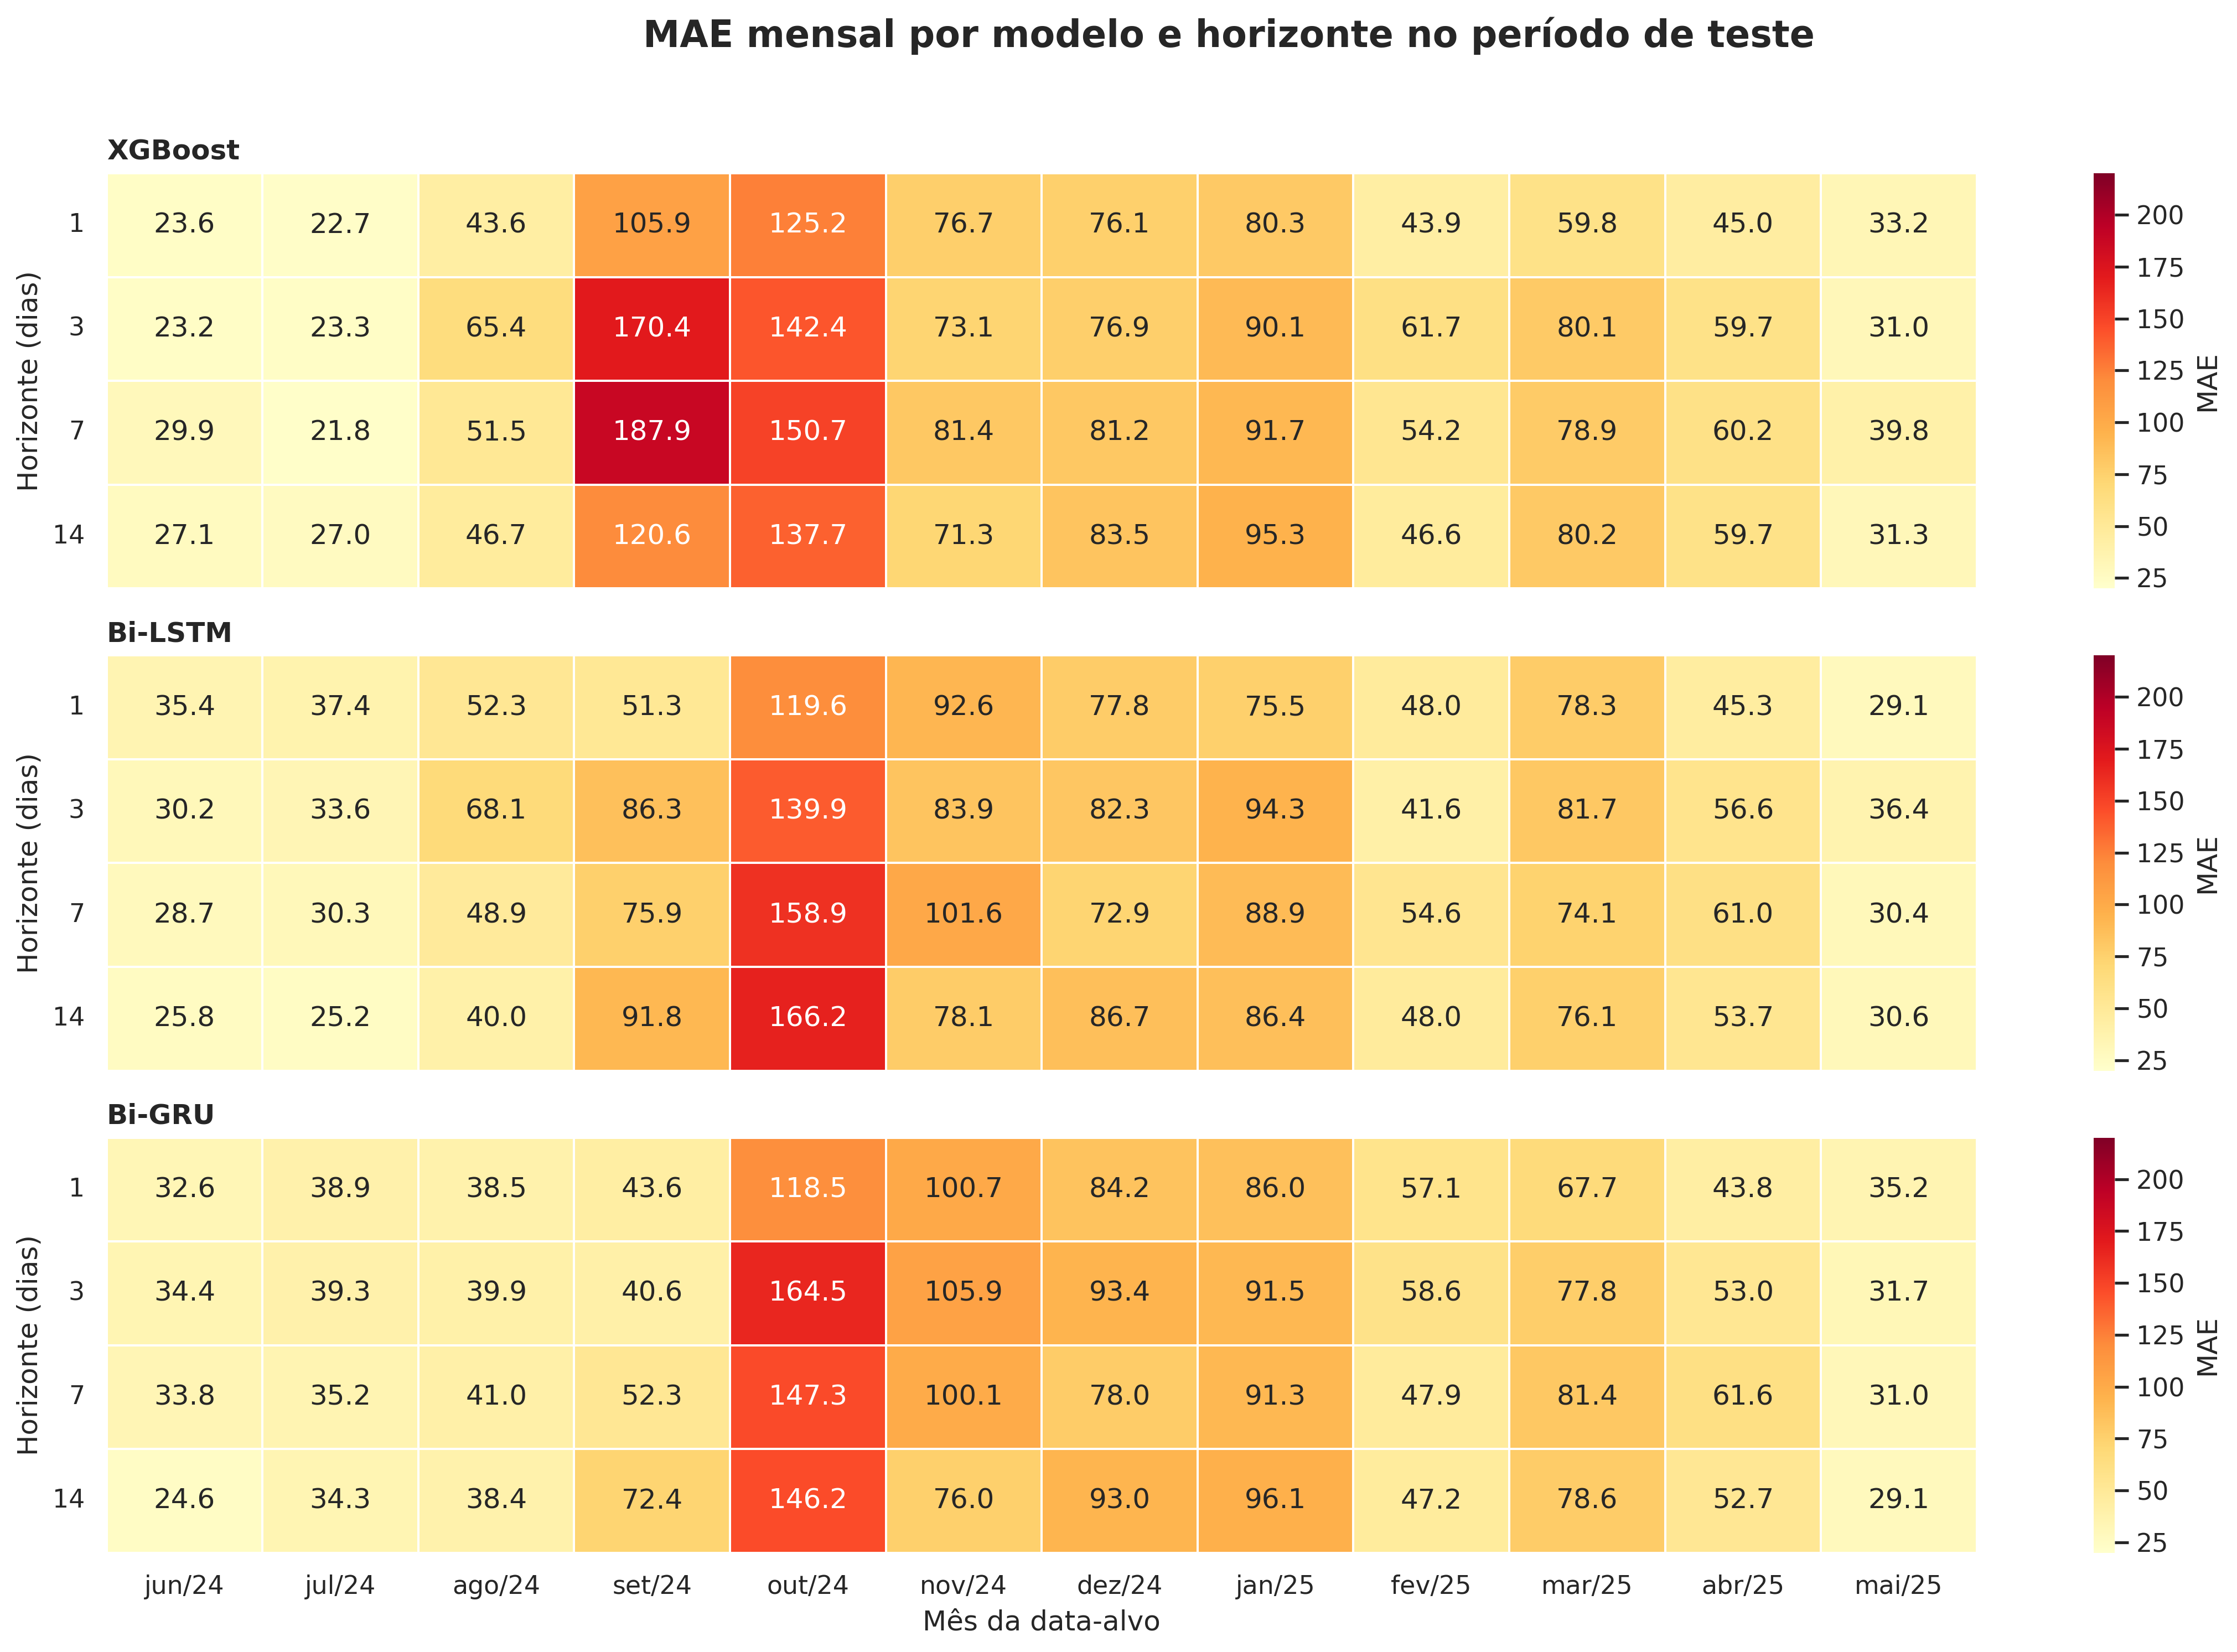
\includegraphics[width=0.78\textwidth]{previsao_multihorizonte_mae_mensal.png}

  \vspace{-0.5em}
  \small
  Setembro e outubro de 2024 formam a janela mais crítica; junho e julho permanecem entre os meses mais estáveis.

  \source{Elaboração dos autores, Figura 4.38.}
  \note{%
    Apresentador: Mateus. Tempo-alvo: 1 minuto e 15 segundos.
    Explicar que a liderança anual varia ao longo dos meses e que os maiores erros coincidem com a transição para a estação chuvosa.
    [Sources] Monografia, Seção 4.10.1 e Figura 4.38; métricas mensais multi-horizonte.
  }
\end{frame}

\begin{frame}{Não existe um único modelo vencedor}{Escolha guiada pela operação}
  \resizebox{0.98\textwidth}{!}{%
    \begin{tabular}{>{\bfseries}p{2.0cm} p{2.6cm} p{5.0cm}}
      \toprule
      Horizonte & Modelo indicado & Uso operacional \\
      \midrule
      1 dia & XGBoost ou Bi-LSTM &
      Alerta de curtíssimo prazo, com boa relação entre erro e custo. \\
      \addlinespace
      3 dias & Bi-LSTM &
      Planejamento de equipes e materiais para a próxima janela operacional. \\
      \addlinespace
      7 e 14 dias & Bi-GRU &
      Preparação logística e acompanhamento preventivo de médio prazo. \\
      \bottomrule
    \end{tabular}%
  }

  \vspace{0.9em}
  \begin{block}{Estratégia recomendada}
    Combinar modelos por horizonte e retrainar periodicamente para acompanhar mudanças na série.
  \end{block}

  \source{Monografia, Seção 5.2.}
  \note{%
    Apresentador: Mateus. Tempo-alvo: 1 minuto e 20 segundos.
    Traduzir o gráfico anterior em decisão. Ressaltar que a escolha depende do horizonte e do custo computacional.
    [Sources] Monografia, Seções 5.2 e 5.7.
  }
\end{frame}

\section{Limitações e aplicação}

\begin{frame}{O escopo dos resultados ainda é restrito}{Limitações}
  \begin{columns}[T,onlytextwidth]
    \begin{column}{0.48\textwidth}
      \textbf{\large Dados}
      \begin{itemize}
        \item Uma única estação meteorológica.
        \item Resolução diária e geografia agregada.
        \item Ausência de topologia, idade dos ativos e vegetação.
      \end{itemize}
    \end{column}
    \begin{column}{0.48\textwidth}
      \textbf{\large Modelagem}
      \begin{itemize}
        \item Apenas 2.687 sequências para as RNNs.
        \item Direção do vento tratada por média simples.
        \item Previsões pontuais sem intervalo de incerteza.
      \end{itemize}
    \end{column}
  \end{columns}

  \vspace{0.8em}
  \begin{block}{Próximos passos}
    Dados horários e espaciais, múltiplas estações, NDVI/LiDAR, índices ENSO e previsão probabilística.
  \end{block}

  \source{Monografia, Seção 5.5 e Capítulo 6.}
  \note{%
    Apresentador: Mateus. Tempo-alvo: 1 minuto e 20 segundos.
    Mostrar domínio crítico do trabalho: não extrapolar causalidade nem generalização nacional.
    [Sources] Monografia, Limitações e Trabalhos Futuros.
  }
\end{frame}

\begin{frame}{A implantação pode começar como alerta}{Caminho para manutenção preditiva}
  \begin{enumerate}
    \item \textbf{Atualizar diariamente} as bases climáticas e operacionais.
    \item \textbf{Gerar previsões por horizonte} com o modelo mais adequado.
    \item \textbf{Acionar limiares} para equipes, materiais e comunicação.
    \item \textbf{Monitorar erro e deriva} e retrainar com dados recentes.
  \end{enumerate}

  \vspace{0.8em}
  \begin{block}{}
    O modelo atua como sistema de alerta: informa a previsão e o horizonte, enquanto a decisão permanece com a operação.
  \end{block}

  \source{Monografia, Seções 5.6 e 6.4.}
  \note{%
    Apresentador: Mateus. Tempo-alvo: 1 minuto.
    Apresentar um caminho incremental, sem prometer automação autônoma da operação.
    [Sources] Monografia, Implicações Práticas e Considerações Finais.
  }
\end{frame}

\section{Conclusão}

\begin{frame}{A melhor arquitetura depende do horizonte}{Conclusões}
  \begin{enumerate}
    \item O clima e o histórico recente contêm \textbf{sinal preditivo relevante}.
    \item Em $h=1$, \textbf{XGBoost e Bi-LSTM} apresentam desempenhos próximos.
    \item Em horizontes maiores, as \textbf{redes recorrentes assumem vantagem}.
    \item Eventos extremos continuam sendo o principal desafio de previsão.
  \end{enumerate}

  \vspace{0.8em}
  \begin{block}{Resposta à pergunta de pesquisa}
    Sim, é possível antecipar interrupções com dados públicos, desde que o modelo seja escolhido pelo horizonte e a incerteza seja considerada.
  \end{block}

  \source{Monografia, Capítulo 6.}
  \note{%
    Apresentador: Mateus. Tempo-alvo: 1 minuto e 20 segundos.
    Retomar a pergunta do início e responder de forma direta.
    [Sources] Monografia, Capítulo 6.
  }
\end{frame}

{\1
\begin{frame}[plain,noframenumbering]
  \finalpage{%
    \begin{center}
      {\Large\bfseries Obrigado!}\\[1.2em]
      {\large Perguntas e discussão}\\[1.8em]
      \small
      Giovanni Minari Zanetti \quad $\cdot$ \quad Mateus Gomes de Araújo
    \end{center}
  }
  \note{%
    Apresentadores: ambos.
    Agradecer à banca e abrir para perguntas.
    [Sources] Não se aplica.
  }
\end{frame}}

% ------------------------------------------------------------------
% SLIDES DE RESERVA PARA A ARGUIÇÃO
% ------------------------------------------------------------------

\appendix

\begin{frame}[noframenumbering]{Métricas completas confirmam a inversão}{Reserva: métricas multi-horizonte}
  \centering
  \scriptsize
  \begin{tabular}{l cc cc cc cc}
    \toprule
     & \multicolumn{2}{c}{$h=1$} & \multicolumn{2}{c}{$h=3$} &
       \multicolumn{2}{c}{$h=7$} & \multicolumn{2}{c}{$h=14$} \\
    \cmidrule(lr){2-3}\cmidrule(lr){4-5}\cmidrule(lr){6-7}\cmidrule(lr){8-9}
    Modelo & MAE & RMSE & MAE & RMSE & MAE & RMSE & MAE & RMSE \\
    \midrule
    XGBoost & 62,46 & 101,41 & 78,77 & 120,02 & 83,83 & 132,10 & 71,34 & 115,23 \\
    Bi-LSTM & 64,19 & 100,44 & 74,01 & 119,47 & 79,49 & 128,40 & 67,69 & 110,24 \\
    Bi-GRU  & 75,10 & 121,18 & 77,67 & 121,77 & 73,61 & 119,92 & 64,31 & 106,27 \\
    \bottomrule
  \end{tabular}

  \vspace{1em}
  \normalsize
  O XGBoost atinge $R^2=-0{,}027$ em $h=7$; a Bi-GRU atinge $R^2=0{,}336$ em $h=14$.

  \source{Arquivo de métricas multi-horizonte do repositório.}
  \note{%
    Slide de reserva.
    [Sources] Monografia, Tabela 4.4; arquivo de métricas multi-horizonte.
  }
\end{frame}

\begin{frame}[noframenumbering]{XGBoost tem menor custo operacional}{Reserva: custo computacional}
  \centering
  \resizebox{0.96\textwidth}{!}{%
    \begin{tabular}{>{\bfseries}p{3.0cm} p{2.3cm} p{2.3cm} p{2.3cm}}
      \toprule
      Critério & XGBoost & Bi-LSTM & Bi-GRU \\
      \midrule
      Parâmetros/nós & $\sim$5.000 nós & 162.433 & 123.905 \\
      Treino em CPU & $<2$ min & $\sim$25 min & $\sim$20 min \\
      GPU & Não & Sim & Sim \\
      Inferência & $<1$ ms/dia & $\sim$5 ms/dia & $\sim$4 ms/dia \\
      Memória & $\sim$50 MB & $\sim$200 MB & $\sim$180 MB \\
      \bottomrule
    \end{tabular}%
  }

  \vspace{1em}
  \begin{block}{Leitura}
    Em $h=1$, o ganho operacional do XGBoost é sua simplicidade; em horizontes longos, a vantagem preditiva das RNNs pode justificar o custo adicional.
  \end{block}

  \source{Estimativas dos experimentos; Monografia, Seção 5.7.}
  \note{%
    Slide de reserva.
    [Sources] Monografia, Tabela 5.3.
  }
\end{frame}

\begin{frame}[noframenumbering]{As redes concentram erros perto de zero}{Reserva: distribuição residual}
  \centering
  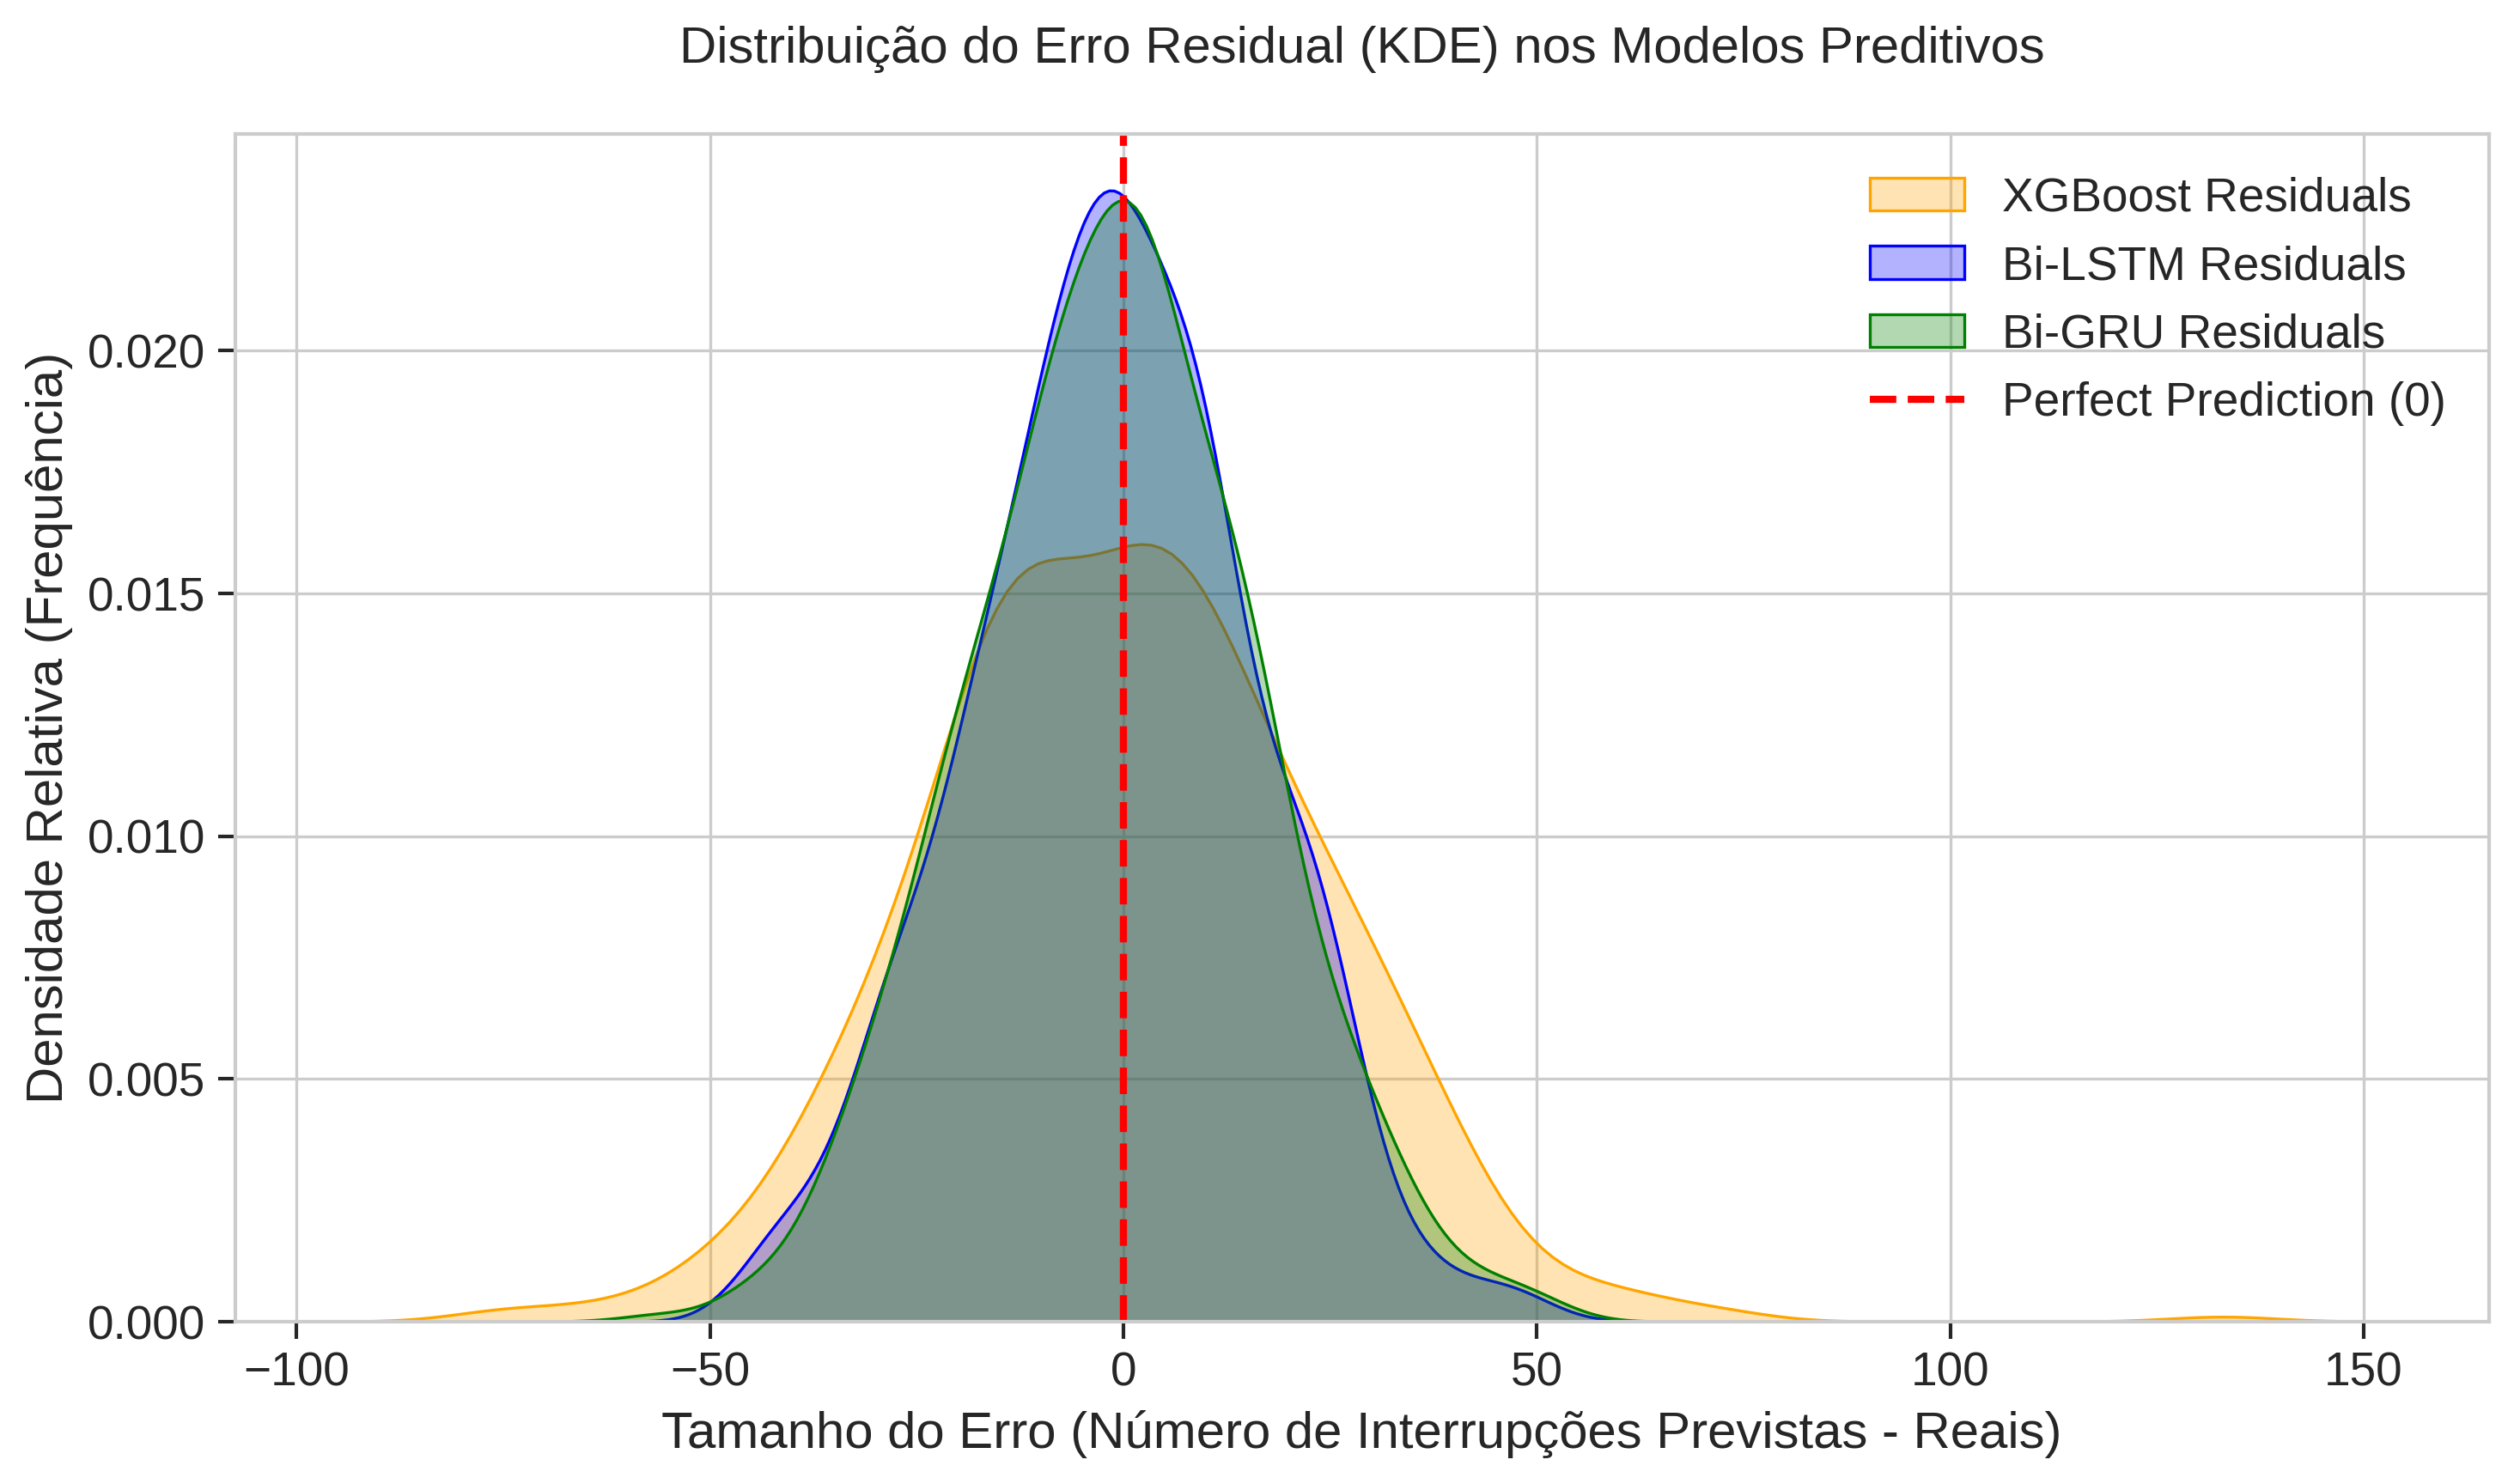
\includegraphics[width=0.83\textwidth]{kde_residuos_modelos.png}

  \vspace{-0.2em}
  \begin{itemize}
    \item Bi-LSTM e Bi-GRU: maior concentração em torno de zero.
    \item XGBoost: distribuição mais achatada e comportamento mais conservador.
  \end{itemize}

  \source{Elaboração dos autores, Figura 4.26.}
  \note{%
    Slide de reserva.
    [Sources] Monografia, Seção 4.5 e Figura 4.26.
  }
\end{frame}

\begin{frame}[noframenumbering]{XGBoost suaviza picos extremos}{Reserva: série multi-horizonte}
  \centering
  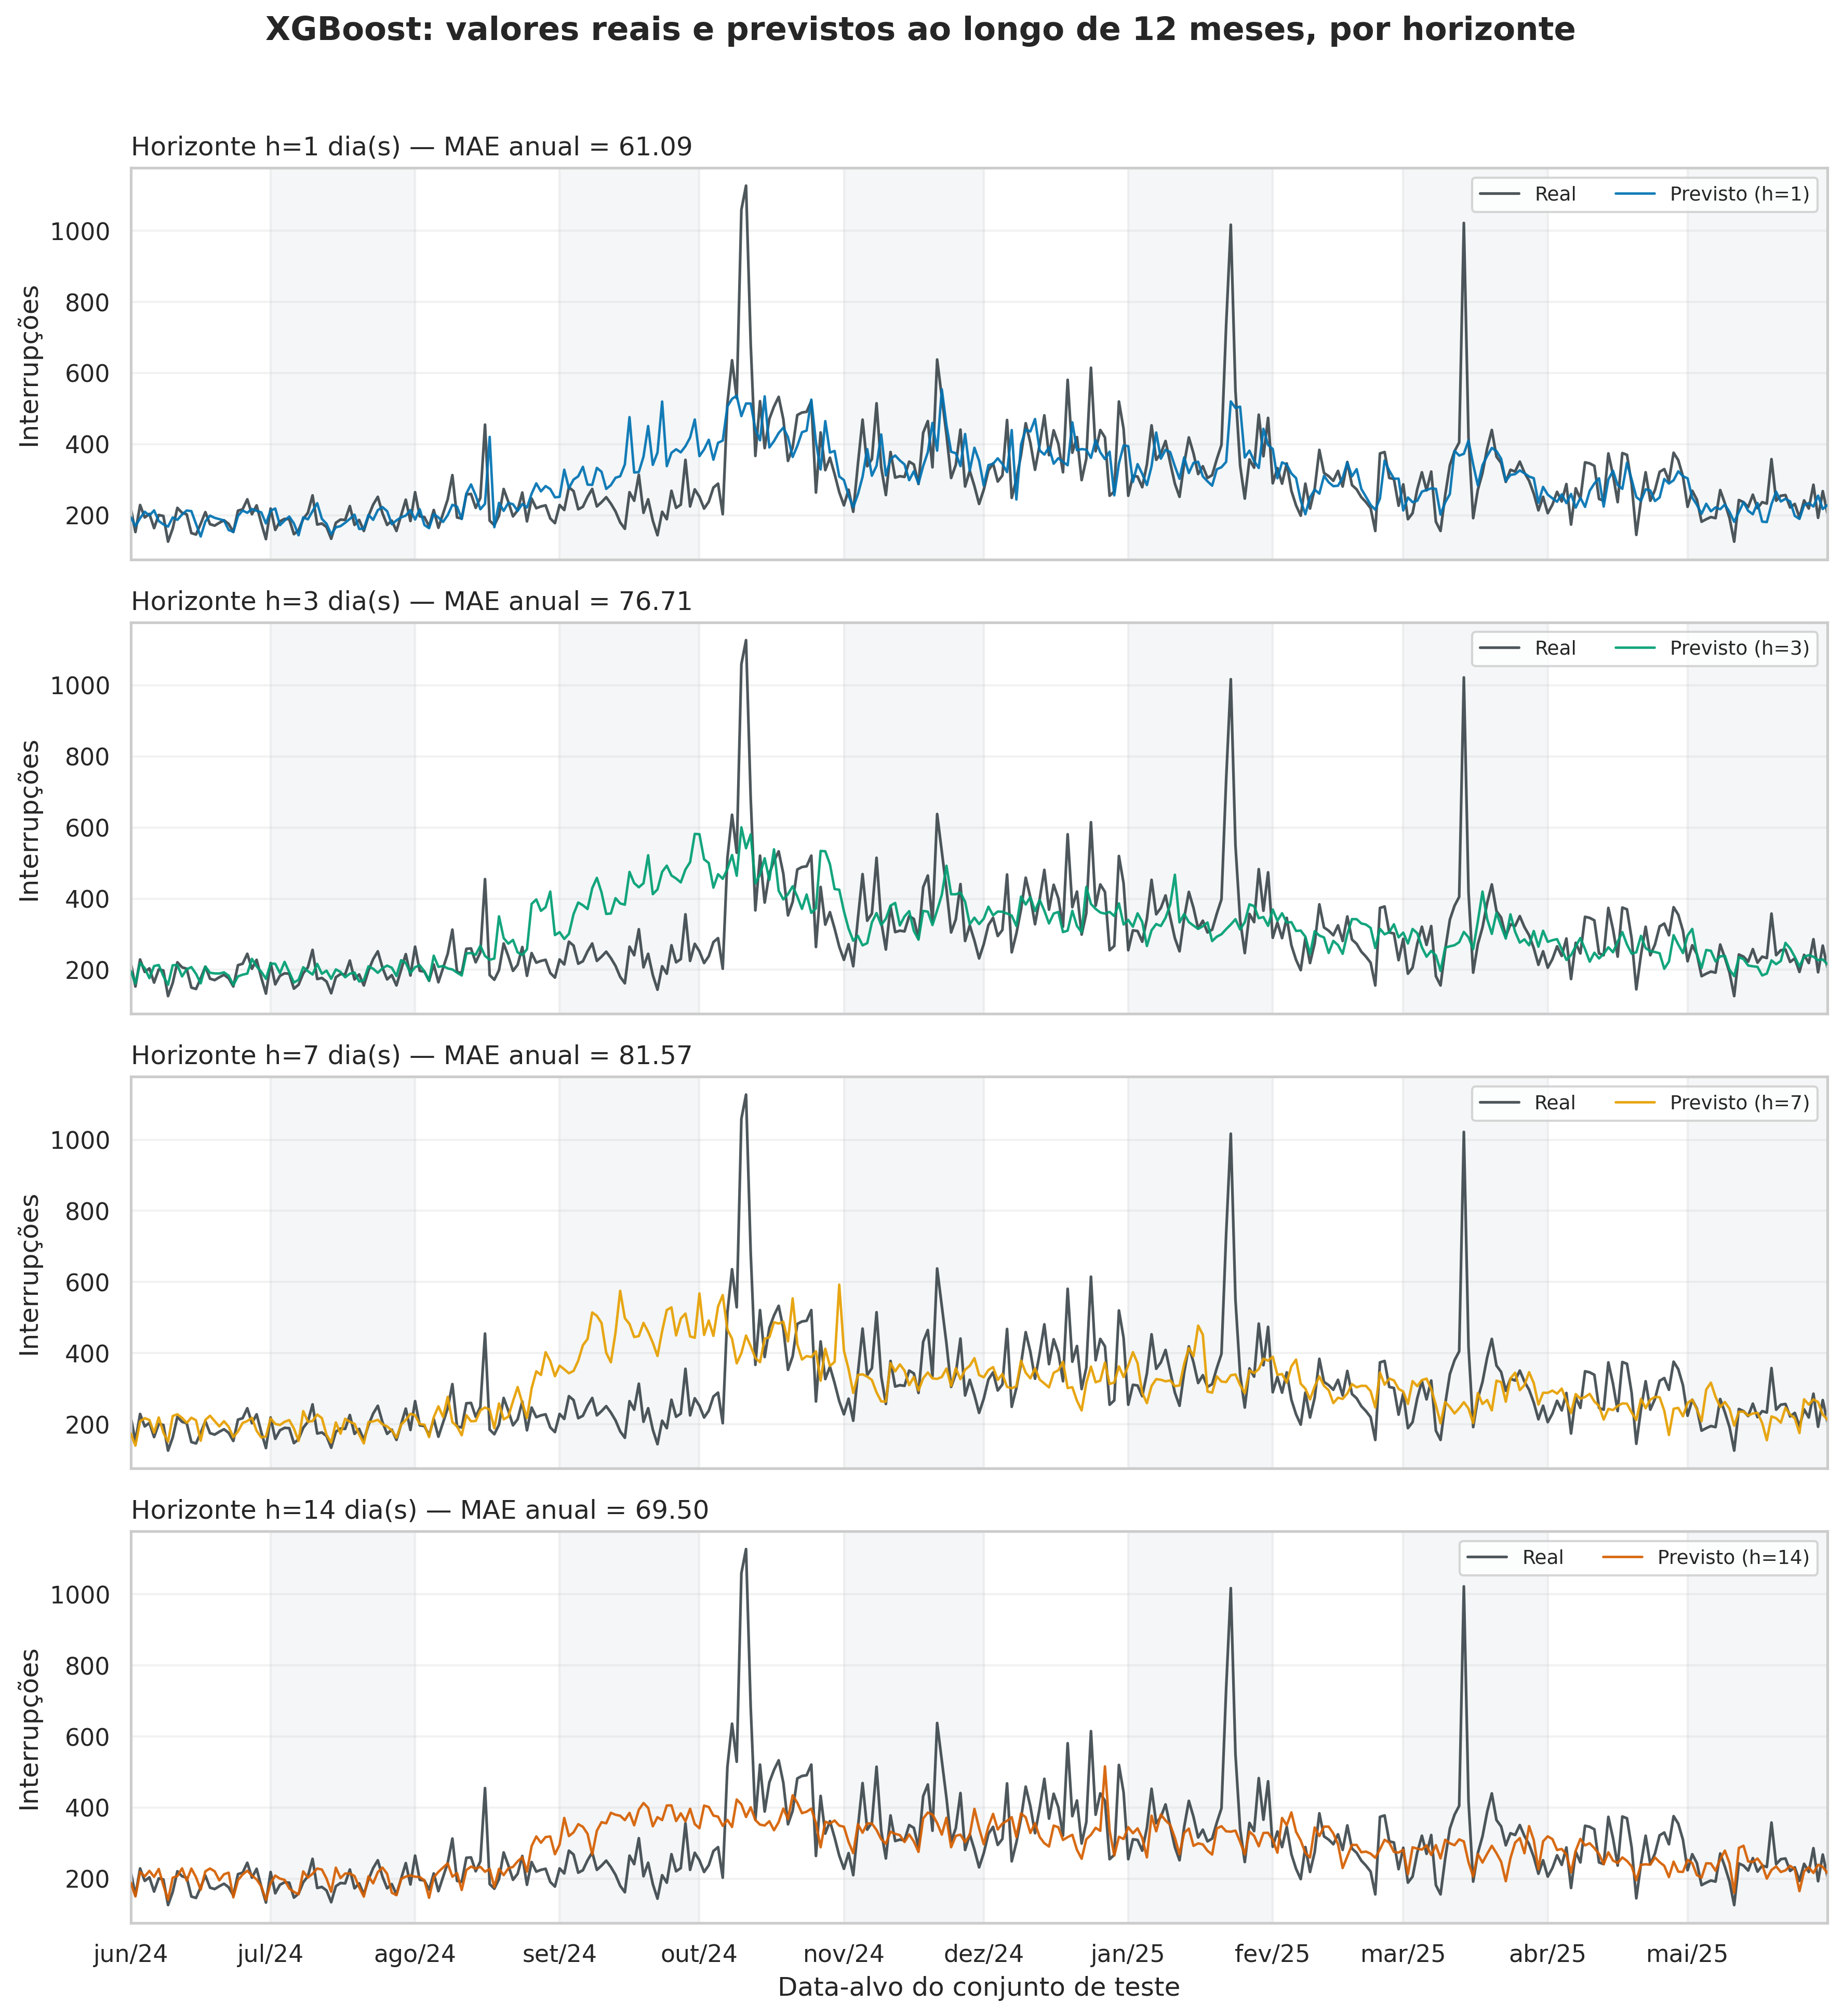
\includegraphics[height=0.72\textheight]{previsao_multihorizonte_temporal_xgboost.png}

  \source{Elaboração dos autores, Figura 4.35.}
  \note{%
    Slide de reserva.
    [Sources] Monografia, Seção 4.10.1 e Figura 4.35.
  }
\end{frame}

\begin{frame}[noframenumbering]{Bi-LSTM suaviza eventos extremos}{Reserva: série multi-horizonte}
  \centering
  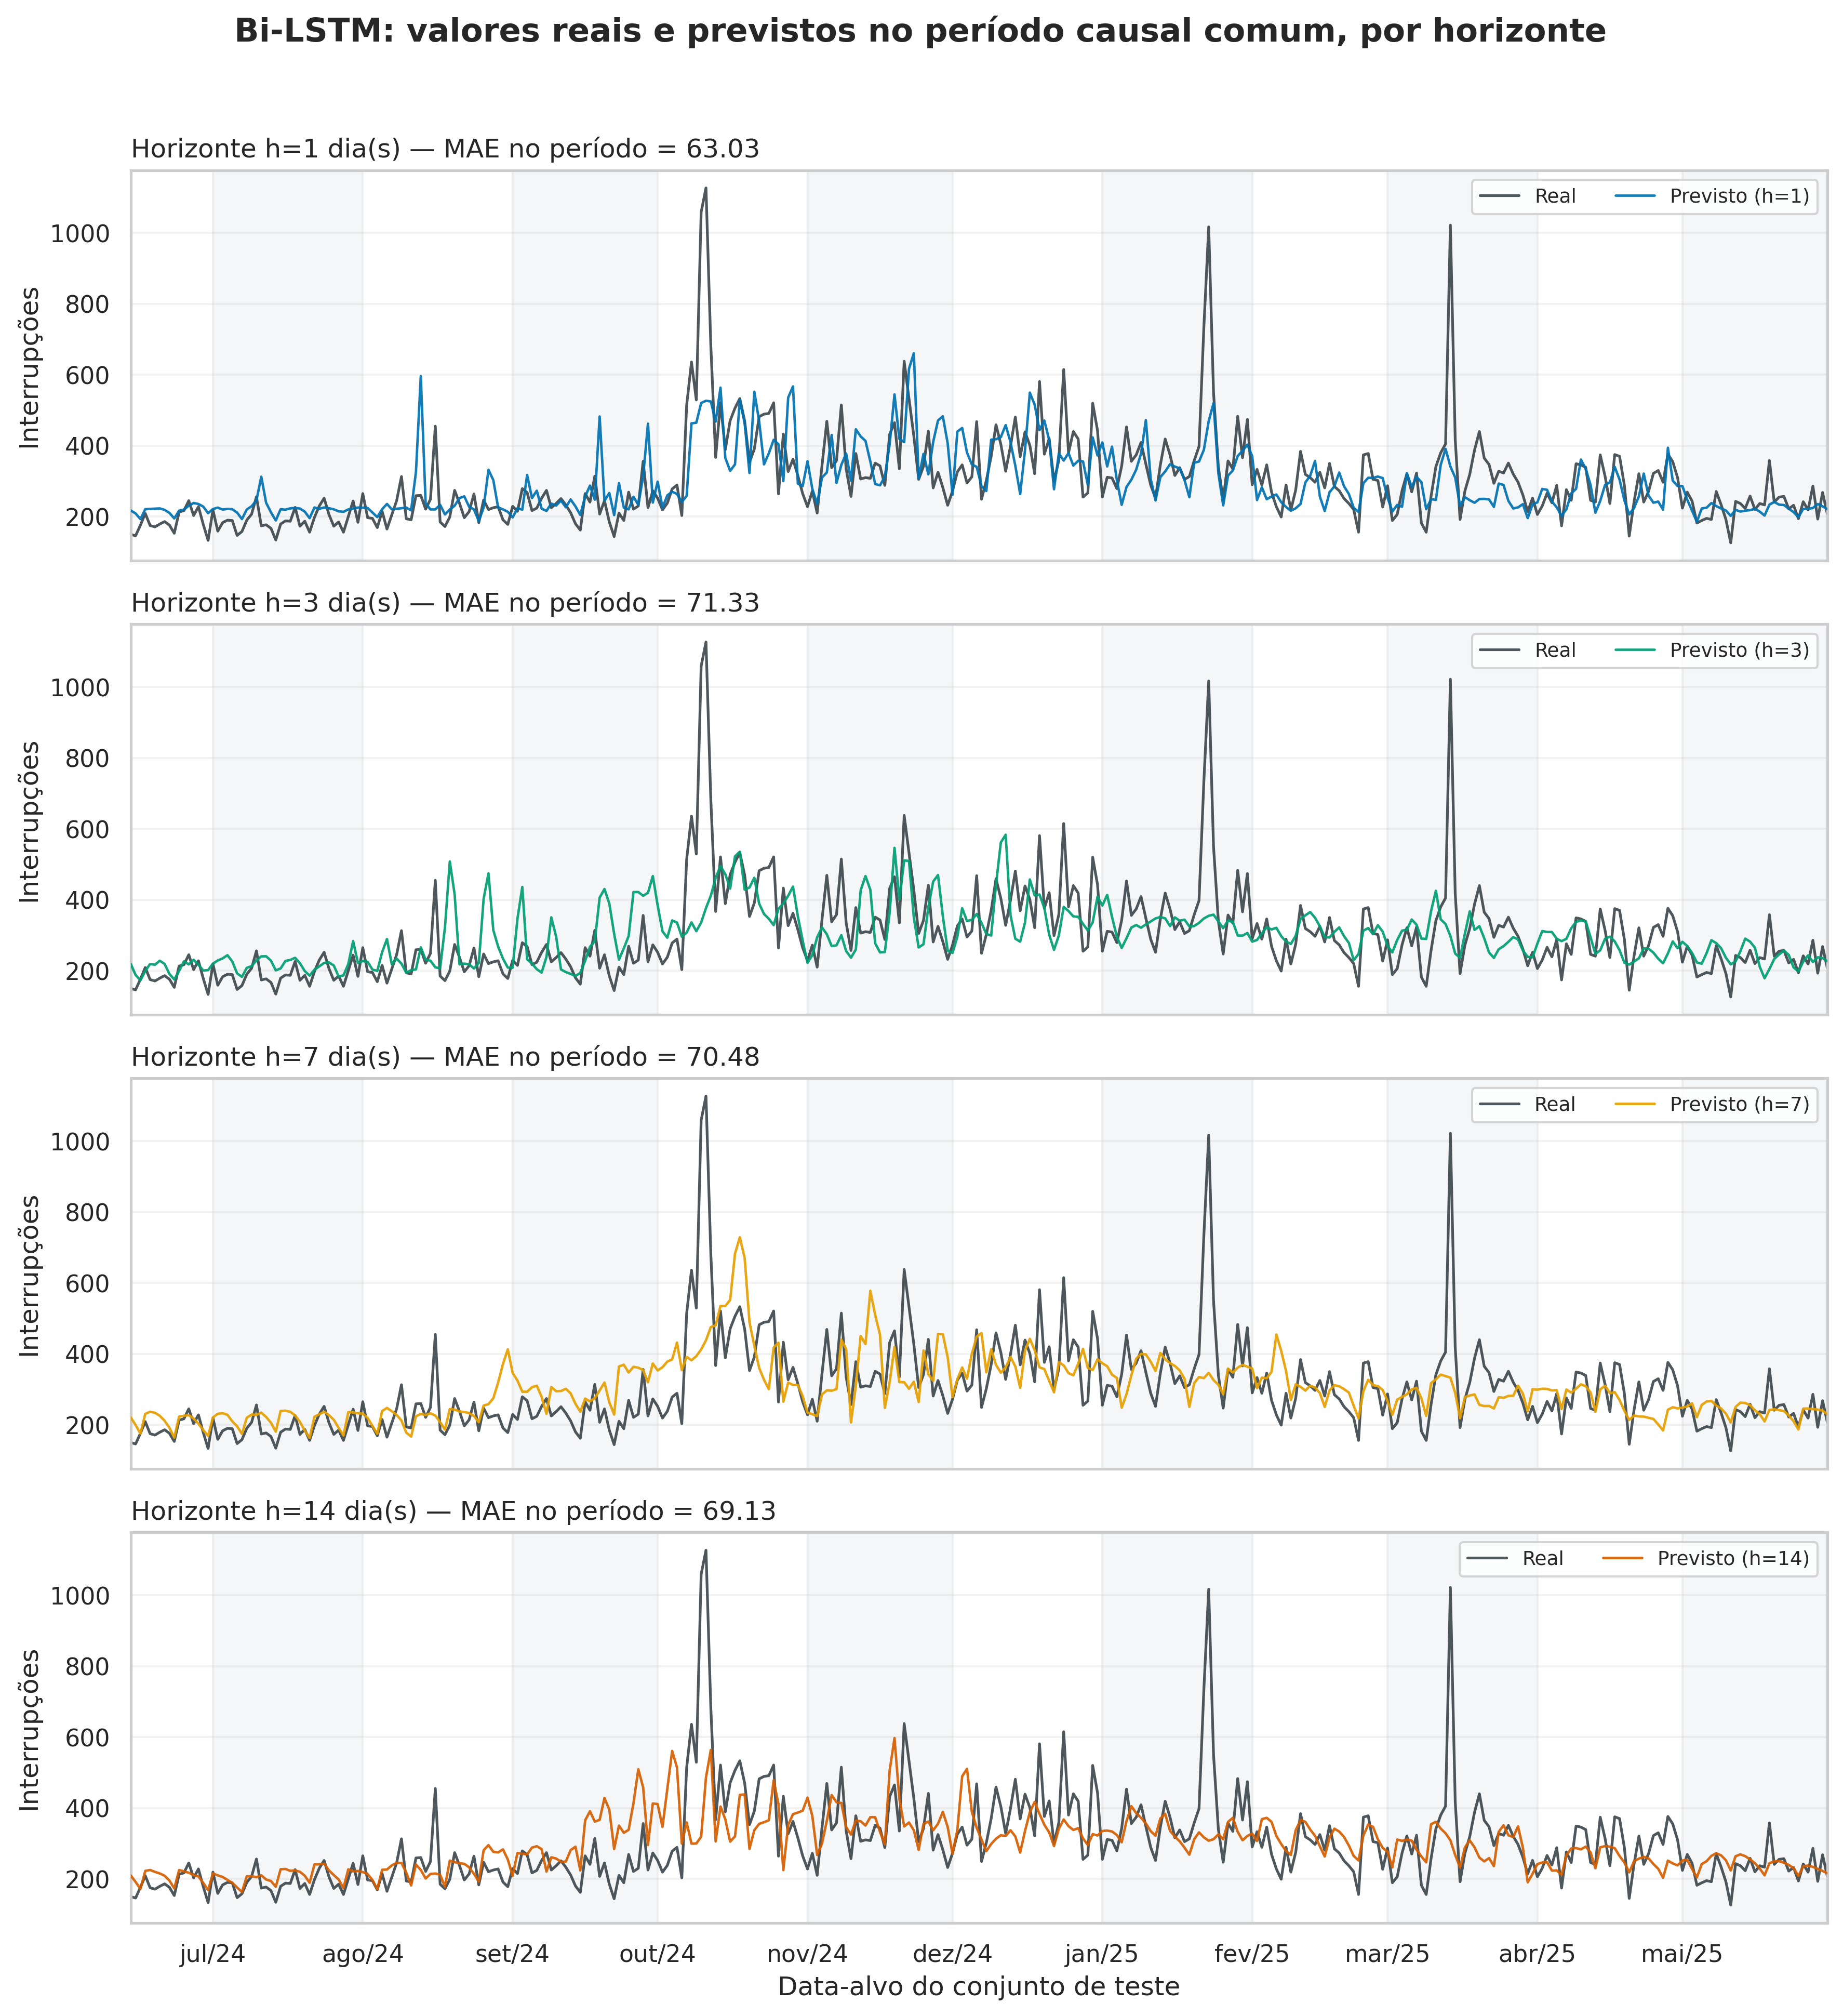
\includegraphics[height=0.72\textheight]{previsao_multihorizonte_temporal_bilstm.png}

  \source{Elaboração dos autores, Figura 4.36.}
  \note{%
    Slide de reserva.
    [Sources] Monografia, Seção 4.10.1 e Figura 4.36.
  }
\end{frame}

\begin{frame}[noframenumbering]{A Bi-GRU ganha vantagem em $h=7$ e $h=14$}{Reserva: série multi-horizonte}
  \centering
  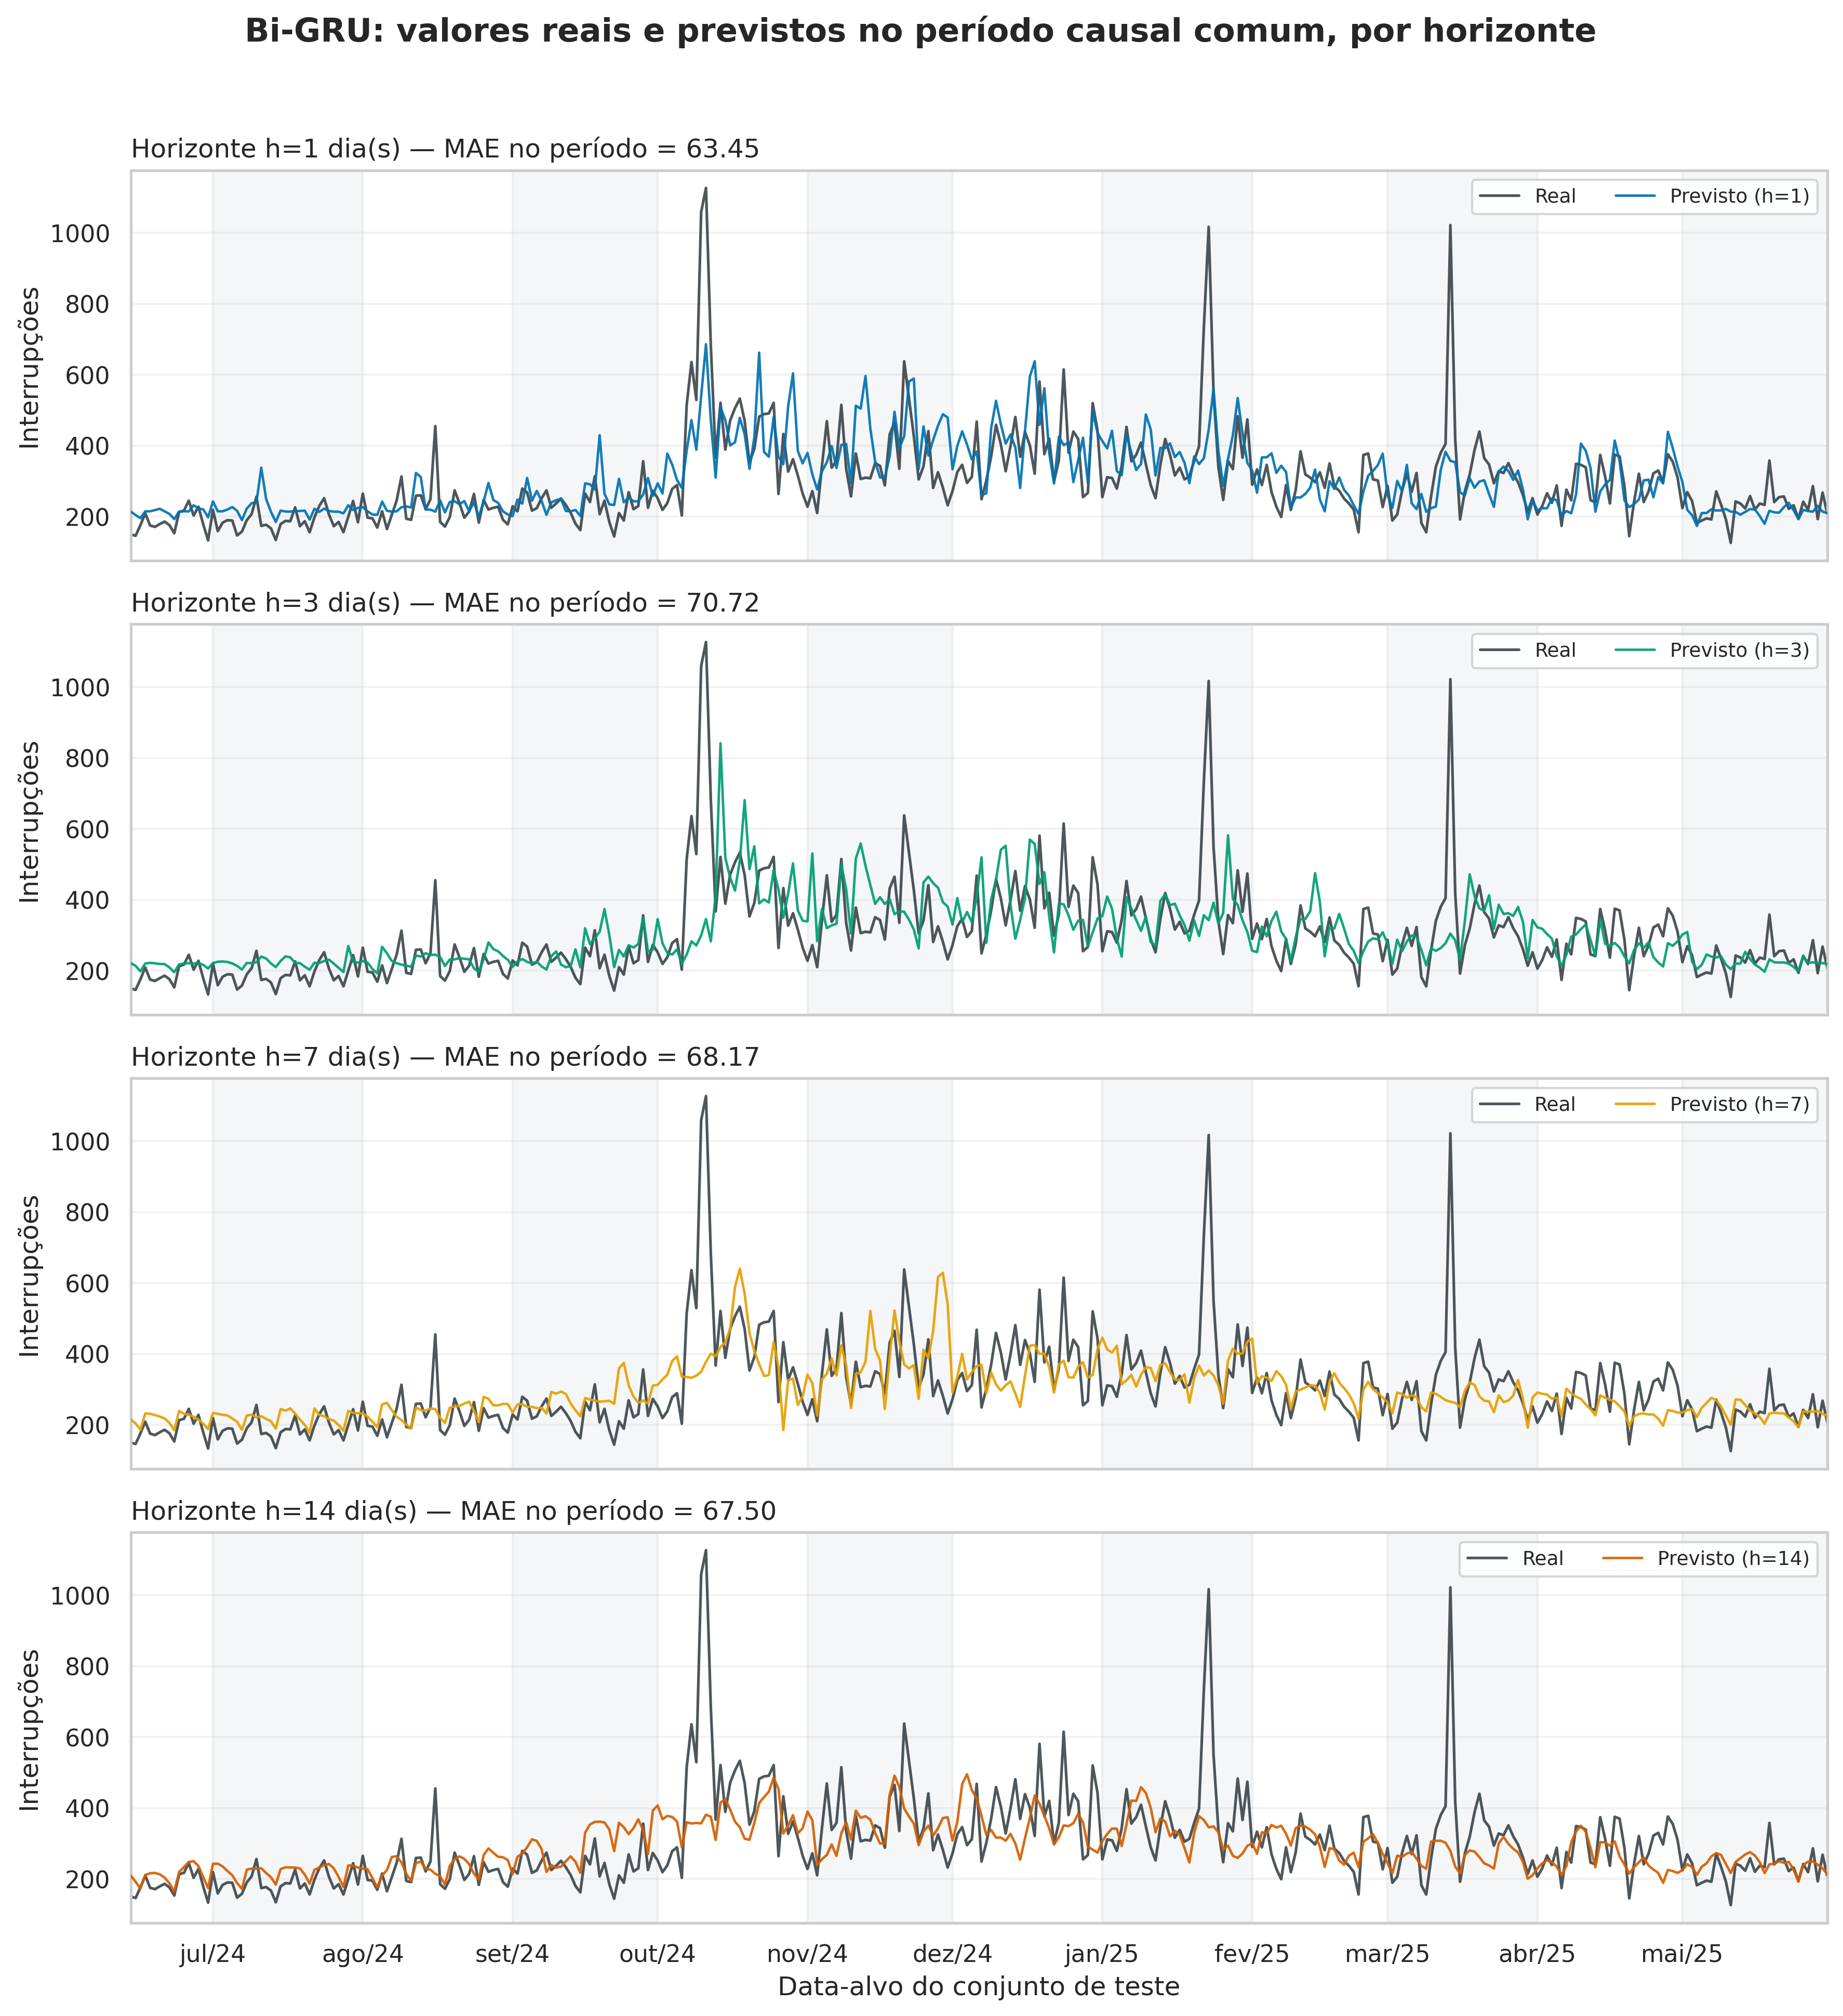
\includegraphics[height=0.72\textheight]{previsao_multihorizonte_temporal_bigru.png}

  \source{Elaboração dos autores, Figura 4.37.}
  \note{%
    Slide de reserva.
    [Sources] Monografia, Seção 4.10.1 e Figura 4.37.
  }
\end{frame}

\begin{frame}[noframenumbering]{O pipeline foi preparado para reprodutibilidade}{Reserva: dados, código e referências}
  \small
  \textbf{Repositório do projeto}\\
  {\scriptsize\url{https://github.com/Mathweuzz/Modelagem-Preditiva-de-Falhas-na-Rede-Eletrica-do-Distrito-Federal}}

  \vspace{0.5em}
  A disponibilização pública integral do código autenticado e dos dados processados está prevista após a conclusão do trabalho.

  \vspace{0.6em}
  \textbf{Fontes de dados}
  \begin{itemize}
    \item INMET -- Dados Históricos, estação A001/Brasília.
    \item ANEEL -- Interrupções de Energia Elétrica nas Redes de Distribuição.
    \item ANEEL/SAMP -- Balanço de energia por mercado.
  \end{itemize}

  \textbf{Referências metodológicas centrais}
  \begin{itemize}
    \item Chen e Guestrin (2016) -- XGBoost.
    \item Hochreiter e Schmidhuber (1997) -- LSTM.
    \item Cho et al. (2014) -- GRU.
  \end{itemize}

  \note{%
    Slide de reserva.
    [Sources] Bibliografia da monografia e repositório do projeto.
  }
\end{frame}

\end{document}
